\documentclass[11pt]{article}

% This file will be kept up-to-date at the following GitHub repository:
%
% https://github.com/automl-conf/LatexTemplate
%
% Please file any issues/bug reports, etc. you may have at:
%
% https://github.com/automl-conf/LatexTemplate/issues

\usepackage{microtype} % microtypography
\usepackage{booktabs}  % tables

% AMS math
\usepackage{amsmath}
\usepackage{amsthm}

% With no package options, the submission will be anonymized, the supplemental
% material will be suppressed, and line numbers will be added to the manuscript.
%
% To hide the supplementary material (e.g., for the first submission deadline),
% use the [hidesupplement] option:
%
% \usepackage[hidesupplement]{automl}
%
% To compile a non-anonymized camera-ready version, add the [final] option:
%
% \usepackage[final]{automl}
%
% or
%
% \usepackage[final, hidesupplement]{automl}

\usepackage[finalworkshop]{automl}

% You may use any reference style as long as you are consistent throughout the
% document. As a default we suggest author--year citations; for bibtex and
% natbib you may use:

\usepackage{natbib}
\bibliographystyle{plain}

% and for biber and biblatex you may use:

% \usepackage[%
%   backend=biber,
%   style=authoryear-comp,
%   sortcites=true,
%   natbib=true,
%   giveninits=true,
%   maxcitenames=2,
%   doi=false,
%   url=true,
%   isbn=false,
%   dashed=false
% ]{biblatex}
% \addbibresource{...}
\usepackage[ruled,linesnumbered]{algorithm2e}
\usepackage{graphicx}
\newcommand\numberthis{\addtocounter{equation}{1}\tag{\theequation}}
\newtheorem{theorem}{Theorem}
\newtheorem{corollary}{Corollary}[theorem]
\newtheorem{lemma}{Lemma}
\usepackage{todonotes}
\usepackage{amssymb}
\usepackage{amsmath}
\usepackage{mathtools}
\usepackage{booktabs}

\newcommand{\floor}[1]{\lfloor #1 \rfloor}

\newcommand{\showcomments}{yes}
\newcommand\jonas[1]{
    \ifthenelse{\equal{\showcomments}{yes}}{{\color{red} Jonas: #1}}{\ignorespaces}
}
\newcommand\xingjian[1]{
    \ifthenelse{\equal{\showcomments}{yes}}{{\color{blue} Xingjian: #1}}{\ignorespaces}}
\newcommand\szha[1]{
    \ifthenelse{\equal{\showcomments}{yes}}{{\color{orange} Sheng: #1}}{\ignorespaces}}
\newcommand*{\affaddr}[1]{#1} % No op here. Customize it for different styles.
\newcommand*{\affmark}[1][*]{\textsuperscript{#1}}
\newcommand*{\email}[1]{\texttt{#1}}
\usepackage[symbol]{footmisc}
\renewcommand{\qedsymbol}{}
\renewcommand{\thefootnote}{\fnsymbol{footnote}}

\title{Towards Automated Distillation: A Systematic Study of Knowledge Distillation in Natural Language Processing}

% Previous title(s): Distiller: A Systematic Study of Knowledge Distillation in Natural Language Processing

% The syntax for adding an author is
%
% \author[i]{\nameemail{author name}{author email}}
%
% where i is an affiliation counter. Authors may have
% multiple affiliations; e.g.:
%
% \author[1,2]{\nameemail{Anonymous}{anonymous@example.com}}

% \author[1]{\nameemail{Author 1}{email1@example.com}}
\author{
Haoyu He\affmark[1] \footnote[2]{Work done while being an intern at Amazon Web Services.}  Xingjian Shi\affmark[2]  Jonas Mueller\affmark[2]  Sheng Zha\affmark[2]  Mu Li\affmark[2]  George Karypis\affmark[2]\\
\affaddr{\affmark[1]Northeastern University} \affaddr{\affmark[2]Amazon Web Services}\\
% \email{he.haoy@northeastern.edu}\\
% \email{\{xjshi,jonasmue,zhasheng,mli,gkarypis\}@amazon.com}\\
}
% the list might continue:
% \author[1]{\nameemail{Haoyu He}{}}
% % \authornote{Work done while being an intern at Amazon Web Services.}
% \author[2]{\nameemail{Xingjian Shi}{}}
% \author[2]{\nameemail{Jonas Mueller}{}}
% \author[2]{\nameemail{Sheng Zha}{}}
% \author[2]{\nameemail{Mu Li}{}}
% \author[2]{\nameemail{George Karypis}{}}
% \author[3]{\nameemail{Author 3}{email3@example.com}}
% \author[4]{\nameemail{Author 4}{email4@example.com}}

% if you need to force a linebreak in the author list, prepend an \author entry
% with \\:

% \author[3]{\\\nameemail{Author 5}{email5@example.com}}

% Specify corresponding affiliations after authors, referring to counter used in
% \author:

% \affil[1]{Institution 1}

% the list might continue:
% \affil[1]{Northeastern University}
% \affil[2]{Amazon Web Services}
% \affil[4]{Institution 4}

% define PDF metadata, please fill in to aid in accessibility of the resulting PDF
\hypersetup{%
  pdfauthor={}, % will be reset to "Anonymous" unless the "final" package option is given
  pdftitle={},
  pdfsubject={},
  pdfkeywords={}
}

\begin{document}

\maketitle

\begin{abstract}
Key factors underpinning the optimal Knowledge Distillation (KD) performance remain elusive as the effects of these factors are often confounded in sophisticated distillation algorithms. This poses a challenge for choosing the best distillation algorithm from the large design space for existing and new tasks alike and hinders automated distillation. In this work, we aim to identify how the distillation performance across different tasks is affected by the components in the KD pipeline, such as the data augmentation policy, the loss function, and the intermediate knowledge transfer between the teacher and the student. To isolate their effects, we propose \emph{Distiller}, a meta-KD framework that systematically combines the key distillation techniques as components across different stages of the KD pipeline. Distiller enables us to quantify each component's contribution and conduct 
experimental studies to derive insights about distillation performance:
1) the approach used to distill the intermediate representations is the most important factor in KD performance,
2) the best-performed distillation algorithms are quite different across various tasks, and
3) data augmentation provides a large boost for small training datasets or small student networks.
Based on these insights, we propose a simple \emph{AutoDistiller} algorithm that can recommend a close-to-optimal KD pipeline for a new dataset/task. This is the first step toward automated KD that can save engineering costs and democratize practical KD applications.
% This is the first step towards automated KD  %for a new dataset based on our findings that different datasets/tasks prefer different KD algorithms.
\end{abstract}
\section{Introduction}

% Recent advancements in Natural Language Processing (NLP) such as  BERT~\cite{devlin2018bert}, RoBERTa~\cite{liu2019roberta}, and ELECTRA~\cite{clark2020electra} have demonstrated the effectiveness of Transformer models in generating transferable language representations. 
% % Pretraining over a massive unlabeled corpus and then fine-tuning over labeled data for the task of interest has become the state-of-the-art paradigm for solving diverse NLP problems ranging from text classification to part-of-speech tagging question answering~\cite{raffel2019exploring}. 
% Scaling up the size of these networks has led to rapid NLP improvements. However, these improvements have come at the expense of significant increase of cost of memory for their many parameters and compute to produce predictions \cite{gpt3,kaplan2020scaling}.
% % attributed to their large model size and high FLOPs, the promising results offered by these pre-trained models come with high computational cost and memory usage. 
% This prevents these models from being deployed on resource-constrained devices such as smart phones and browsers, or for latency-constrained applications such as click-through-rate prediction. There is great demand for models that are smaller in size, yet still retain similar accuracy as those having a large number of parameters. %, which is critical for  application in broader scenarios.

% Pretrained language models excel in representing general knowledge and adapting to downstream natural language processing (NLP) tasks, yet the high inference cost of the giant models hinders them from being deployed on resource-constrained devices such as smart phones and browsers.
To reduce the inference cost while preserving most of the accuracy of prevalent large pretrained models used in natural language processing (NLP), \emph{task-aware} KD is a popular and particularly promising approach for supervised learning tasks. The idea is to first fine-tune an accurate and large \emph{teacher} model on the labeled data, and then train a separate \emph{student} model that has much fewer parameters to mimic the predictions of the teacher. Innovations in KD for NLP generally improve the following aspects: 1) the loss function for gauging the discrepancy between student and teacher predictions, 2) the method for transferring intermediate network representations between teacher and student, 3) the use of data augmentation during student training, and 4) multiple stages of  distillation. Many studies have simultaneously introduced new variations of more than one of these components, which confounds the impact of each component on the final performance of the distillation algorithm. In addition, it is often unclear whether the proposed KD algorithms retain their advantageous performance across different tasks besides those they are evaluated on. As a result, selecting the solution from the large combined design space of KD algorithms for a new application is increasingly challenging. This is a major obstacle for \emph{automated KD}, of which the goal is to recommend a good KD pipeline for a new dataset.
% An automated KD system that recommends KD algorithm per dataset.
% For example, MixKD~\cite{liang2020mixkd} has only been evaluated on classification problems and it is unclear if the method will be effective for question answering.
%Moreover, important phenomena regarding KD for NLP remain unexplained, such as the observation by \citet{sun2019patient} that distilling from a larger teacher can make the student perform worse in some down-stream tasks. Much popular KD work~\cite{li2020bert,sanh2019distilbert} chose to distill from the BERT-base model and has not  investigated if their proposed methods still perform well for larger teachers. 


To understand the importance of different components in KD and lay the cornerstone for automated KD, we conduct a systematic study of the design space of KD algorithms in NLP. We compose several key configurable components in KD into a meta-distillation pipeline, called \emph{Distiller}. All candidate algorithms in the search space of \emph{Distiller} work for two main types of NLP tasks: text classification and sentence tagging. We run extensive hyper-parameter tuning algorithms to search for the best \emph{Distiller}-configuration choices over GLUE~\citep{wang2018glue} and SQuAD~\citep{rajpurkar2016squad}. The hyper-parameter search helps us understand what impact different KD components have on student performance and motivates us to propose \emph{AutoDistiller} as the very first step towards automated KD that can save engineering cost and democratize machine learning. \emph{AutoDistiller} is designed to predict distillation performance based on KD pipeline choices and characteristics of tasks. We expect our proposed AutoDistiller, as a baseline of automated KD, to bring fresh insights to the rapidly growing automated machine learning (AutoML) community. Experimental analysis of \emph{AutoDistiller} shows that it is potential to reliably prioritize high-performing KD configurations, and can suggest good distillation pipelines on two new datasets. Main contributions of this work are:


\begin{itemize}
    \item A systematic study on the meta-KD pipeline \emph{Distiller} to assess the impact of different components in KD, including the: 1) data augmentation policy, 2) loss function for transferring intermediate representations, 3) layer mapping strategies for intermediate representations, 4) loss function for transferring outputs, as well as what role the task and dataset type play.
    % \item Unification of existing objectives for distilling intermediate representations as instances of maximizing the bounds of the mutual information between teacher and student representations. 
    % A unifying perspective on existing objectives for distilling intermediate representations as all maximizing the mutual information between teacher and student representations. Based on this unification, we propose 
    % This leads us to propose  
    % the MI-$\alpha$ objective that outperforms the existing objectives.
    \item Using experimental results collected from our \emph{Distiller} study and features extracted from downstream datasets, we fit a model that automatically predicts the best distillation strategy for new datasets. On hold-out datasets ``BoolQ''~\citep{wang2019superglue} and ``cloth'',  predicted strategies achieve $0.99$ and $0.14$ distillation ratios (fraction of the student's and teacher's performance enhancement gained from distillation) on average, outperforming randomly selected strategies with mean of -$0.98$ and -$0.24$. To the best of our knowledge, this is the first attempt toward automated KD in NLP, providing a baseline solution to future automated KD study.
\end{itemize}
\vspace{-1em}
\section{Related Work}
\label{related work}
\paragraph{Knowledge Distillation}
% The general KD framework was popularized by \citet{bucilua2006model,hinton2015distilling}, aiming to transfer knowledge from an accurate but cumbersome teacher model to a compact student model by matching the class probabilities produced by the teacher and the student. 
In the domain of NLP, recent KD literature discussed how to transfer knowledge from pretrained Transformer-based models efficiently. \citep{sun2019patient} proposed BERT-PKD that transfers the knowledge from both the final layer and intermediate layers of the teacher network. \citep{jiao2019tinybert} proposed TinyBERT that first distills the general knowledge of the teacher by minimizing the Masked Language Model (MLM) objective~\citep{devlin2018bert}, followed by task-specific distillation. \citep{li2020bert} proposed a many-to-many layer mapping function leveraging the Earth Mover’s Distance to transfer intermediate knowledge. \citep{hou2020dynabert} proposed DynaBERT, a multistage distillation pipeline to distill the teacher Transformer to student Transformer with different widths and depths. Focusing on AutoML settings with tabular data, \citep{fakoor2020fast} proposed a general KD algorithm for different classical ML models and ensembles thereof.
% Also hoping to identify good choices in the KD pipeline like our work,
\citep{kim2021comparing} compared Kullback-Leibler divergence and mean squared error objectives in KD for image classification models, finding that the mean squared error performs better. 
\cite{textbrewer-acl2020-demo} introduced an open-source KD toolkit that supports various KD techniques.
% \citet{mukherjee-hassan-awadallah-2020-xtremedistil} also considered multistage KD pipelines with a focus on multilingual Named Entity Recognition. 
% \citet{xu2021bert} proposed NAS-BERT which leverages neural architecture search to train a big super-network that can output multiple compressed models with adaptive sizes and latency. 
%Our paper differs from the existing work in that we provide a systematic analysis of the different components in  single-stage task-aware KD algorithms in NLP . Moreover, we propose the first automated KD algorithm in this area, as well as the use of mutual information objectives for intermediate representation distillation.
Our work provides a systematic analysis of the different components in  single-stage task-aware KD algorithms in NLP and propose the first automated KD algorithm in this area.

% Thus, our considered DA module is similar to  AutoAugment~\citep{cubuk2019autoaugment}, except it is used for KD in NLP with different elementary operators. \szha{I'm not sure if it's necessary to make this comparison. We are studying the effect of data augmentation, not building a general-purpose augmentation framework.}
\vspace{-0.5em}
\section{Methodology}

\label{methodology}
Our study is structured around a configurable meta-distillation pipeline called \emph{Distiller}\footnote[1]{The complete training and testing code are available at https://github.com/Cli212/Distiller.} (details in Appendix \ref{sec:distiller}). It contains four configurable components: the data augmentation policy $a(\cdot, \cdot)$, the layer mapping configuration of intermediate distillation $\{m_{i, j}\}$,  the intermediate distillation objective  $l^{\text{inter}}(\cdot,\cdot)$, and the prediction layer distillation objective $l^{\text{pred}}(\cdot,\cdot)$. Assume the teacher network $f^T$ has $M$ layers and the student network $f^S$ has $N$ layers, for a given data/label pair $(x,y)$ sampled from the dataset $\mathcal{D}$, the student learns from the teacher by minimizing loss: 
\begin{footnotesize}
\begin{equation}
\label{eq:objective}
\begin{aligned}
    \mathcal{L} = \mathbb{E}_{\hat{x}, \hat{y} \sim a(x, y); x, y \sim \mathcal{D}} \sum_{i=1}^M \sum_{j=1}^N m_{i,j}l_{i,j}^{\text{inter}}(H_i^{\text{T}},H_j^{\text{S}})
    &+ \beta_1 l^{\text{pred}}(f^{T}(x),f^{S}(x))
    + \beta_2 l^{\text{pred}}(f^{T}(\hat{x}),f^{S}(\hat{x}))\\
    &+ \gamma_1 l^{\text{pred}}(y, f^{S}(x)) 
    + \gamma_2 l^{\text{pred}}(\hat{y}, f^{S}(\hat{x})).
\end{aligned}
\end{equation}
\end{footnotesize}

Here, $m_{i, j} \in [0, 1]$ represents the layer mapping weight between the $i$-th teacher layer and $j$-th student layer, $H_i^\text{T}, H_j^\text{S}$ are the $i$-th and the $j$-th layer of hidden representations of the teacher and the student, $\beta_1$, $\beta_2$ control the strength of distilling from class probabilities produced by the teacher, and $\gamma_1$, $\gamma_2$ control the strength of learning from ground truth data ($x,y$) and synthesized data ($\hat{x},\hat{y}$). In Appendix \ref{subsec:distiller_search_space}, we illustrate how previous model distillation algorithms~\citep{jiao2019tinybert, li2020bert, liang2020mixkd} can be encompassed in the Distiller framework.
% We next discuss possible design choices for each component and also introduce the AutoDistiller.
\begin{figure}[tb!]
  \centering
  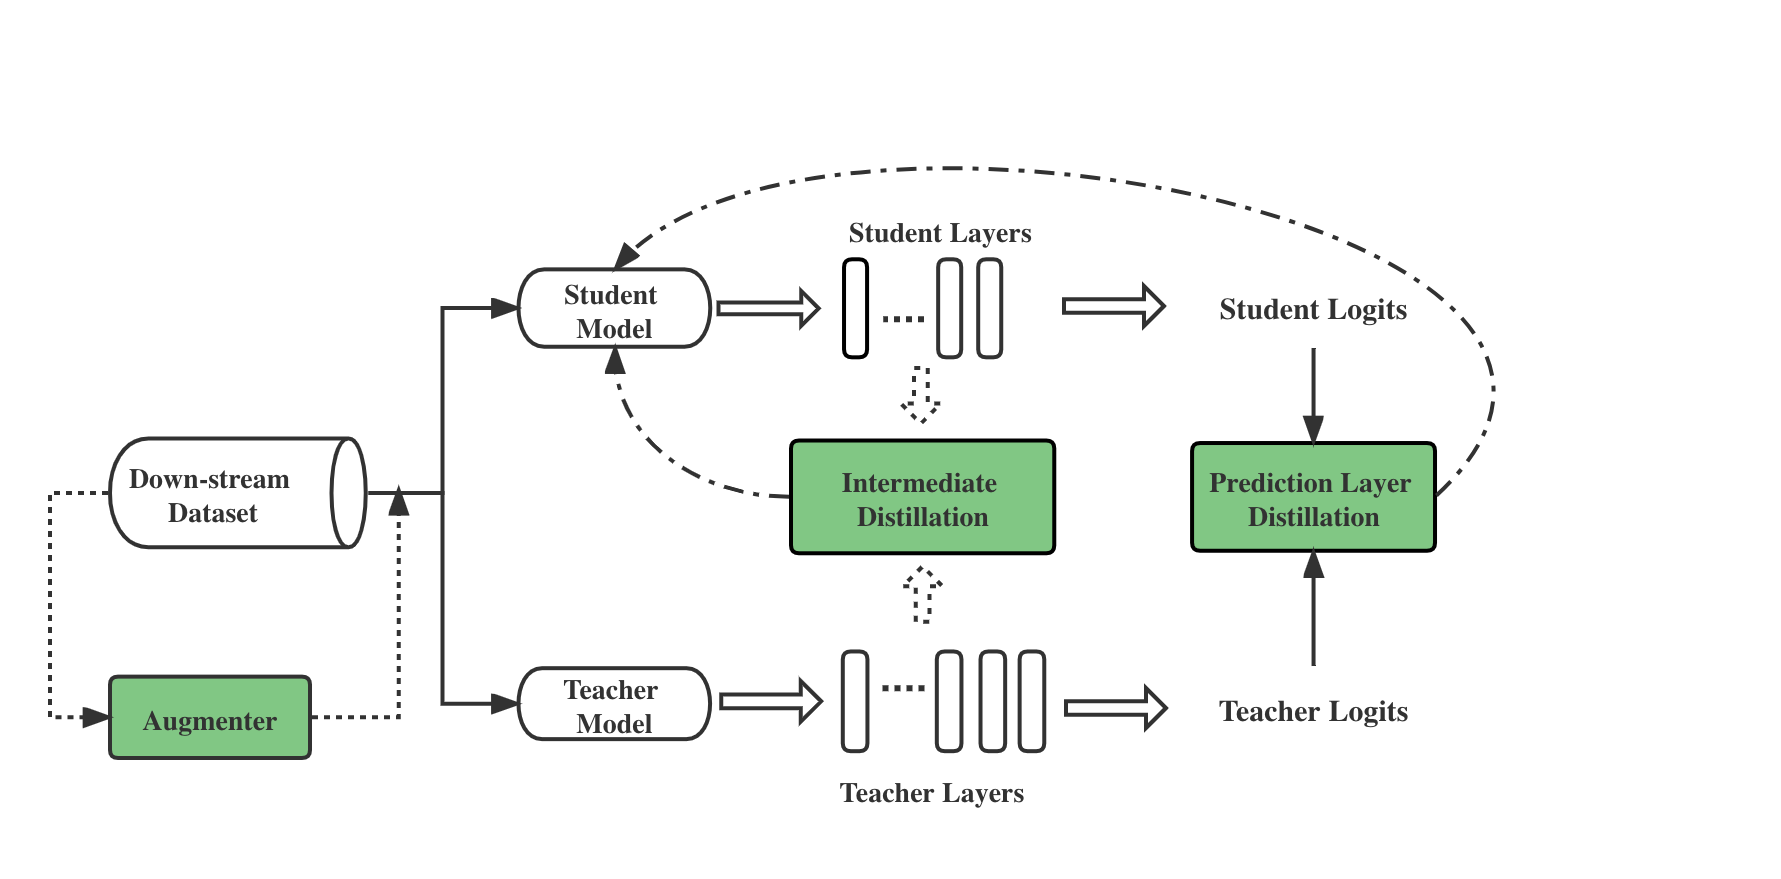
\includegraphics[width=0.5\textwidth]{pics/Distiller.png}
%   \vspace{-1em}
  \caption{Overview of the \emph{Distiller} pipeline. All configurable components are colored.}
%   \vspace{-1em}
%   Augmenter is the data augmentation component. Intermediate distillation covers intermediate layer mapping strategy and intermediate objective. Prediction layer distillation calculates KD loss of the student output and teacher output.
\end{figure}




\subsection{AutoDistiller}
To enable automated distillation, we fit a prediction model that recommends a good KD pipeline based on the features extracted from the dataset and Distiller search space. To encode semantic information of the dataset into features, the context and dataset descriptions are further represented by aggregated GloVe \citep{pennington2014glove} embeddings of words weighted by TF-IDF. We also extract numerical features such as the finetuned baseline score and the finetuned teacher score to measure how tough the task is in need of a complex network, and the number of samples in the dataset. Details about dataset feature extraction are described in Table \ref{tab:task_embedding} in Appendix. To effectively measure the performance enhancement gained by distillation over finetuning, \emph{AutoDistiller} is trained to predict the \textbf{distillation ratio}:
\begin{footnotesize}
\begin{equation}
    r=\frac{S_\textsuperscript{distill}-S_\textsuperscript{finetune}}{T_\textsuperscript{finetune}-S_\textsuperscript{finetune}},
\end{equation}
\end{footnotesize}

where $S_\textsuperscript{distill}$ is the evaluation score of the distilled student, $T_\textsuperscript{finetune}, S_\textsuperscript{finetune}$ are evaluation scores of finetuned student and teacher. This allows us to clearly represent how much performance improvement the student gains from distillation rather than finetuning from scratch. Besides, this ratio can be used across different tasks and different teacher/student architectures so we can continuously update \emph{AutoDistiller} by feeding more distillation results in the future. Once trained on features extracted from datasets as well as features of each candidate distillation configuration, \emph{AutoDistiller} recommends distillation pipelines that maximize the predicted distillation ratio given any downstream dataset/task. To the best of our knowledge, \emph{AutoDistiller} is the first attempt toward automated KD in NLP.
\label{sec:autodistiller}
% \vspace{-1em}
\section{Experiments}
\label{sec:experiments}

Under the previously described experimental setup, we conduct experiments and collect more than 1300 sets of data points that include \emph{Distiller} configuration, the dataset/task, and distillation results. Analyzing the data reveals three major findings: 1) design of the intermediate distillation module is the most important among all factors studied, 2) DA provides a large boost when the dataset or the student model is small, and 3) the best distillation policy varies among datasets. Detailed experimental results revealed these three findings can be found in Appendix \ref{additional_results}. Inspired by these findings, we train a meta-learning model \emph{AutoDistiller} that is able to recommend a good distillation policy on a new dataset based on which configurations tended to work well for alike datasets applied in our study.

\subsection{Importance of Components}
To study the importance of each component described in the previous section, we randomly sample \emph{Distiller} configurations in the designed search space while controlling the optimizer and other unrelated hyper-parameters. We apply each sampled distillation configuration on a diverse set of NLP tasks and different teacher/student architectures. To analyze the importance of different components in \emph{Distiller}, we adopt fANOVA~\citep{hutter2014efficient}, an algorithm for quantifying the importance of individual hyper-parameters as well as their interactions in determining downstream performance. We use fANOVA to evaluate the importance of the four components in \emph{Distiller} as well as their pairwise combinations: data augmentation, intermediate distillation objective, layer mapping strategy, and prediction layer distillation objective. We report the results in Figure \ref{fig:fanova}, which illustrates that the objective function for intermediate distillation $l^{\text{pred}}$ has the highest individual importance, and the combination of the intermediate distillation objective and layer mapping strategy has the highest joint importance. One hypothetical explanation is that the teacher can provide token-level supervision to the student via intermediate distillation, which can better guide the learning process of the student. Therefore, one should most critically focus on these two components when selecting or designing a particular KD pipeline. 

\begin{figure*}[!tb]
    \centering
    \begin{subfigure}[b]{0.4\textwidth}
    \centering
    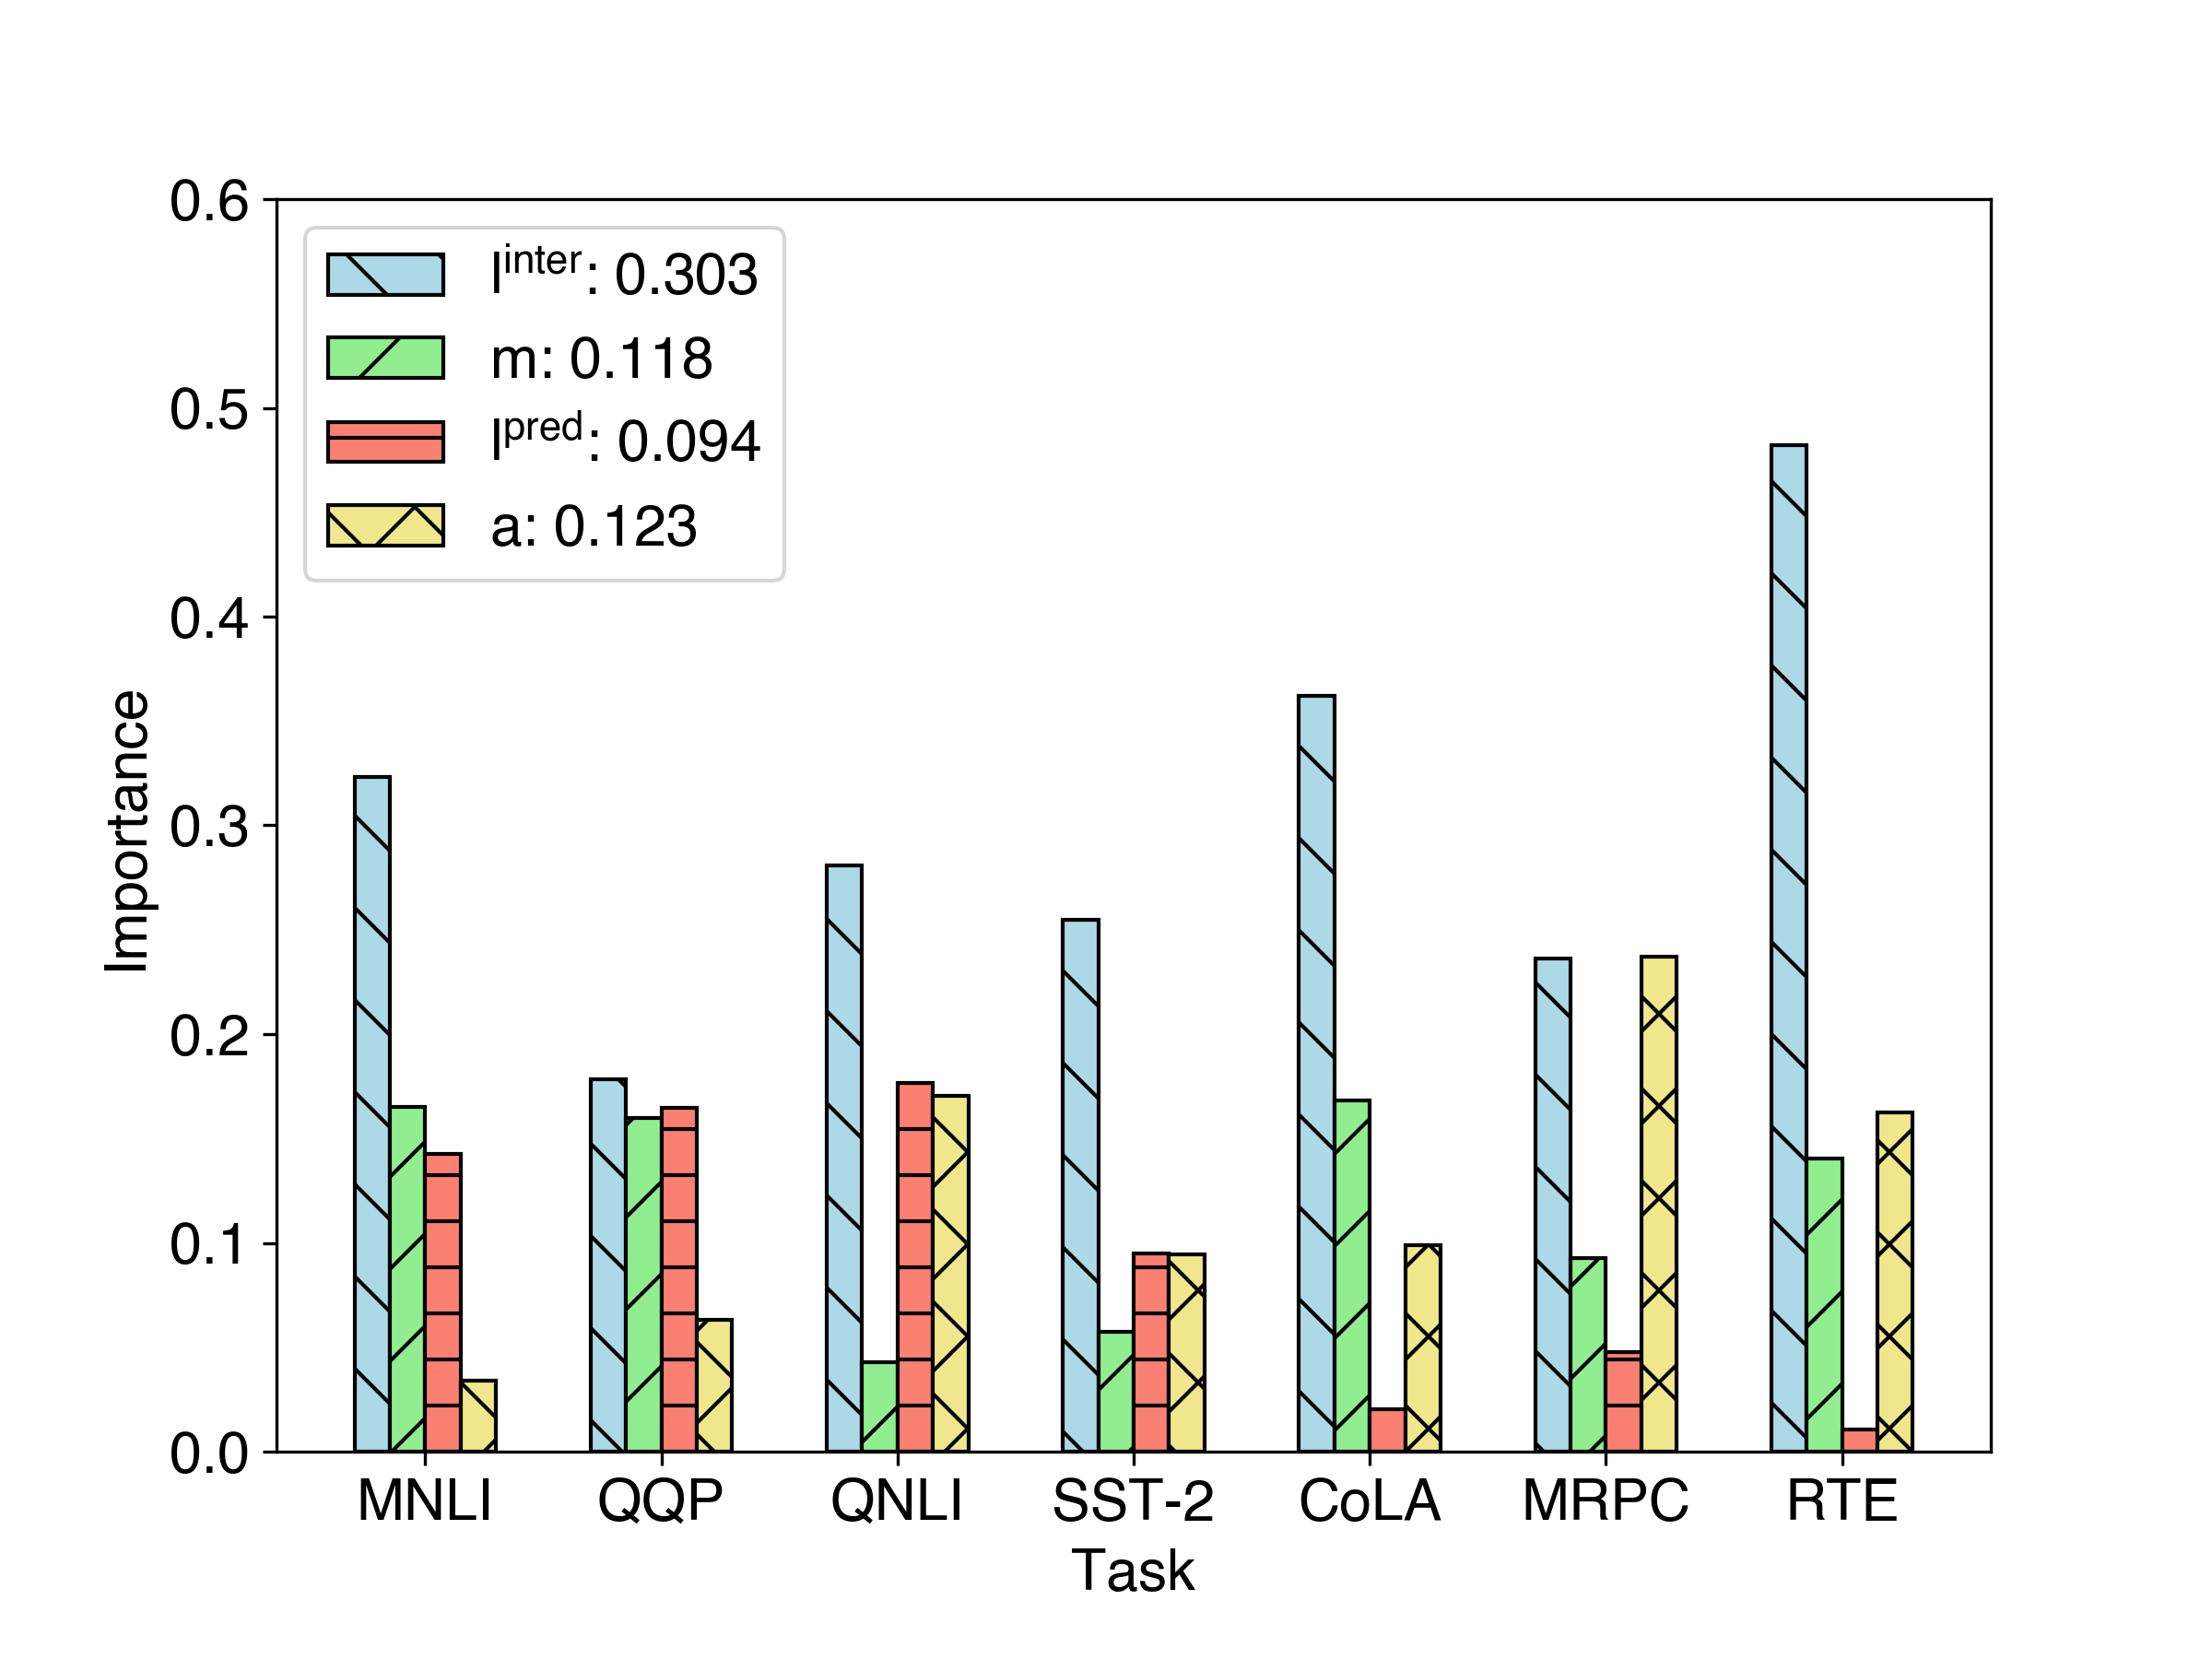
\includegraphics[width=1.0\textwidth]{pics/fanova_single_wo_stsb.png}
    \caption{}
    \end{subfigure}
    \begin{subfigure}[b]{0.4\textwidth}
%    \begin{minipage}{6cm}
    \centering
    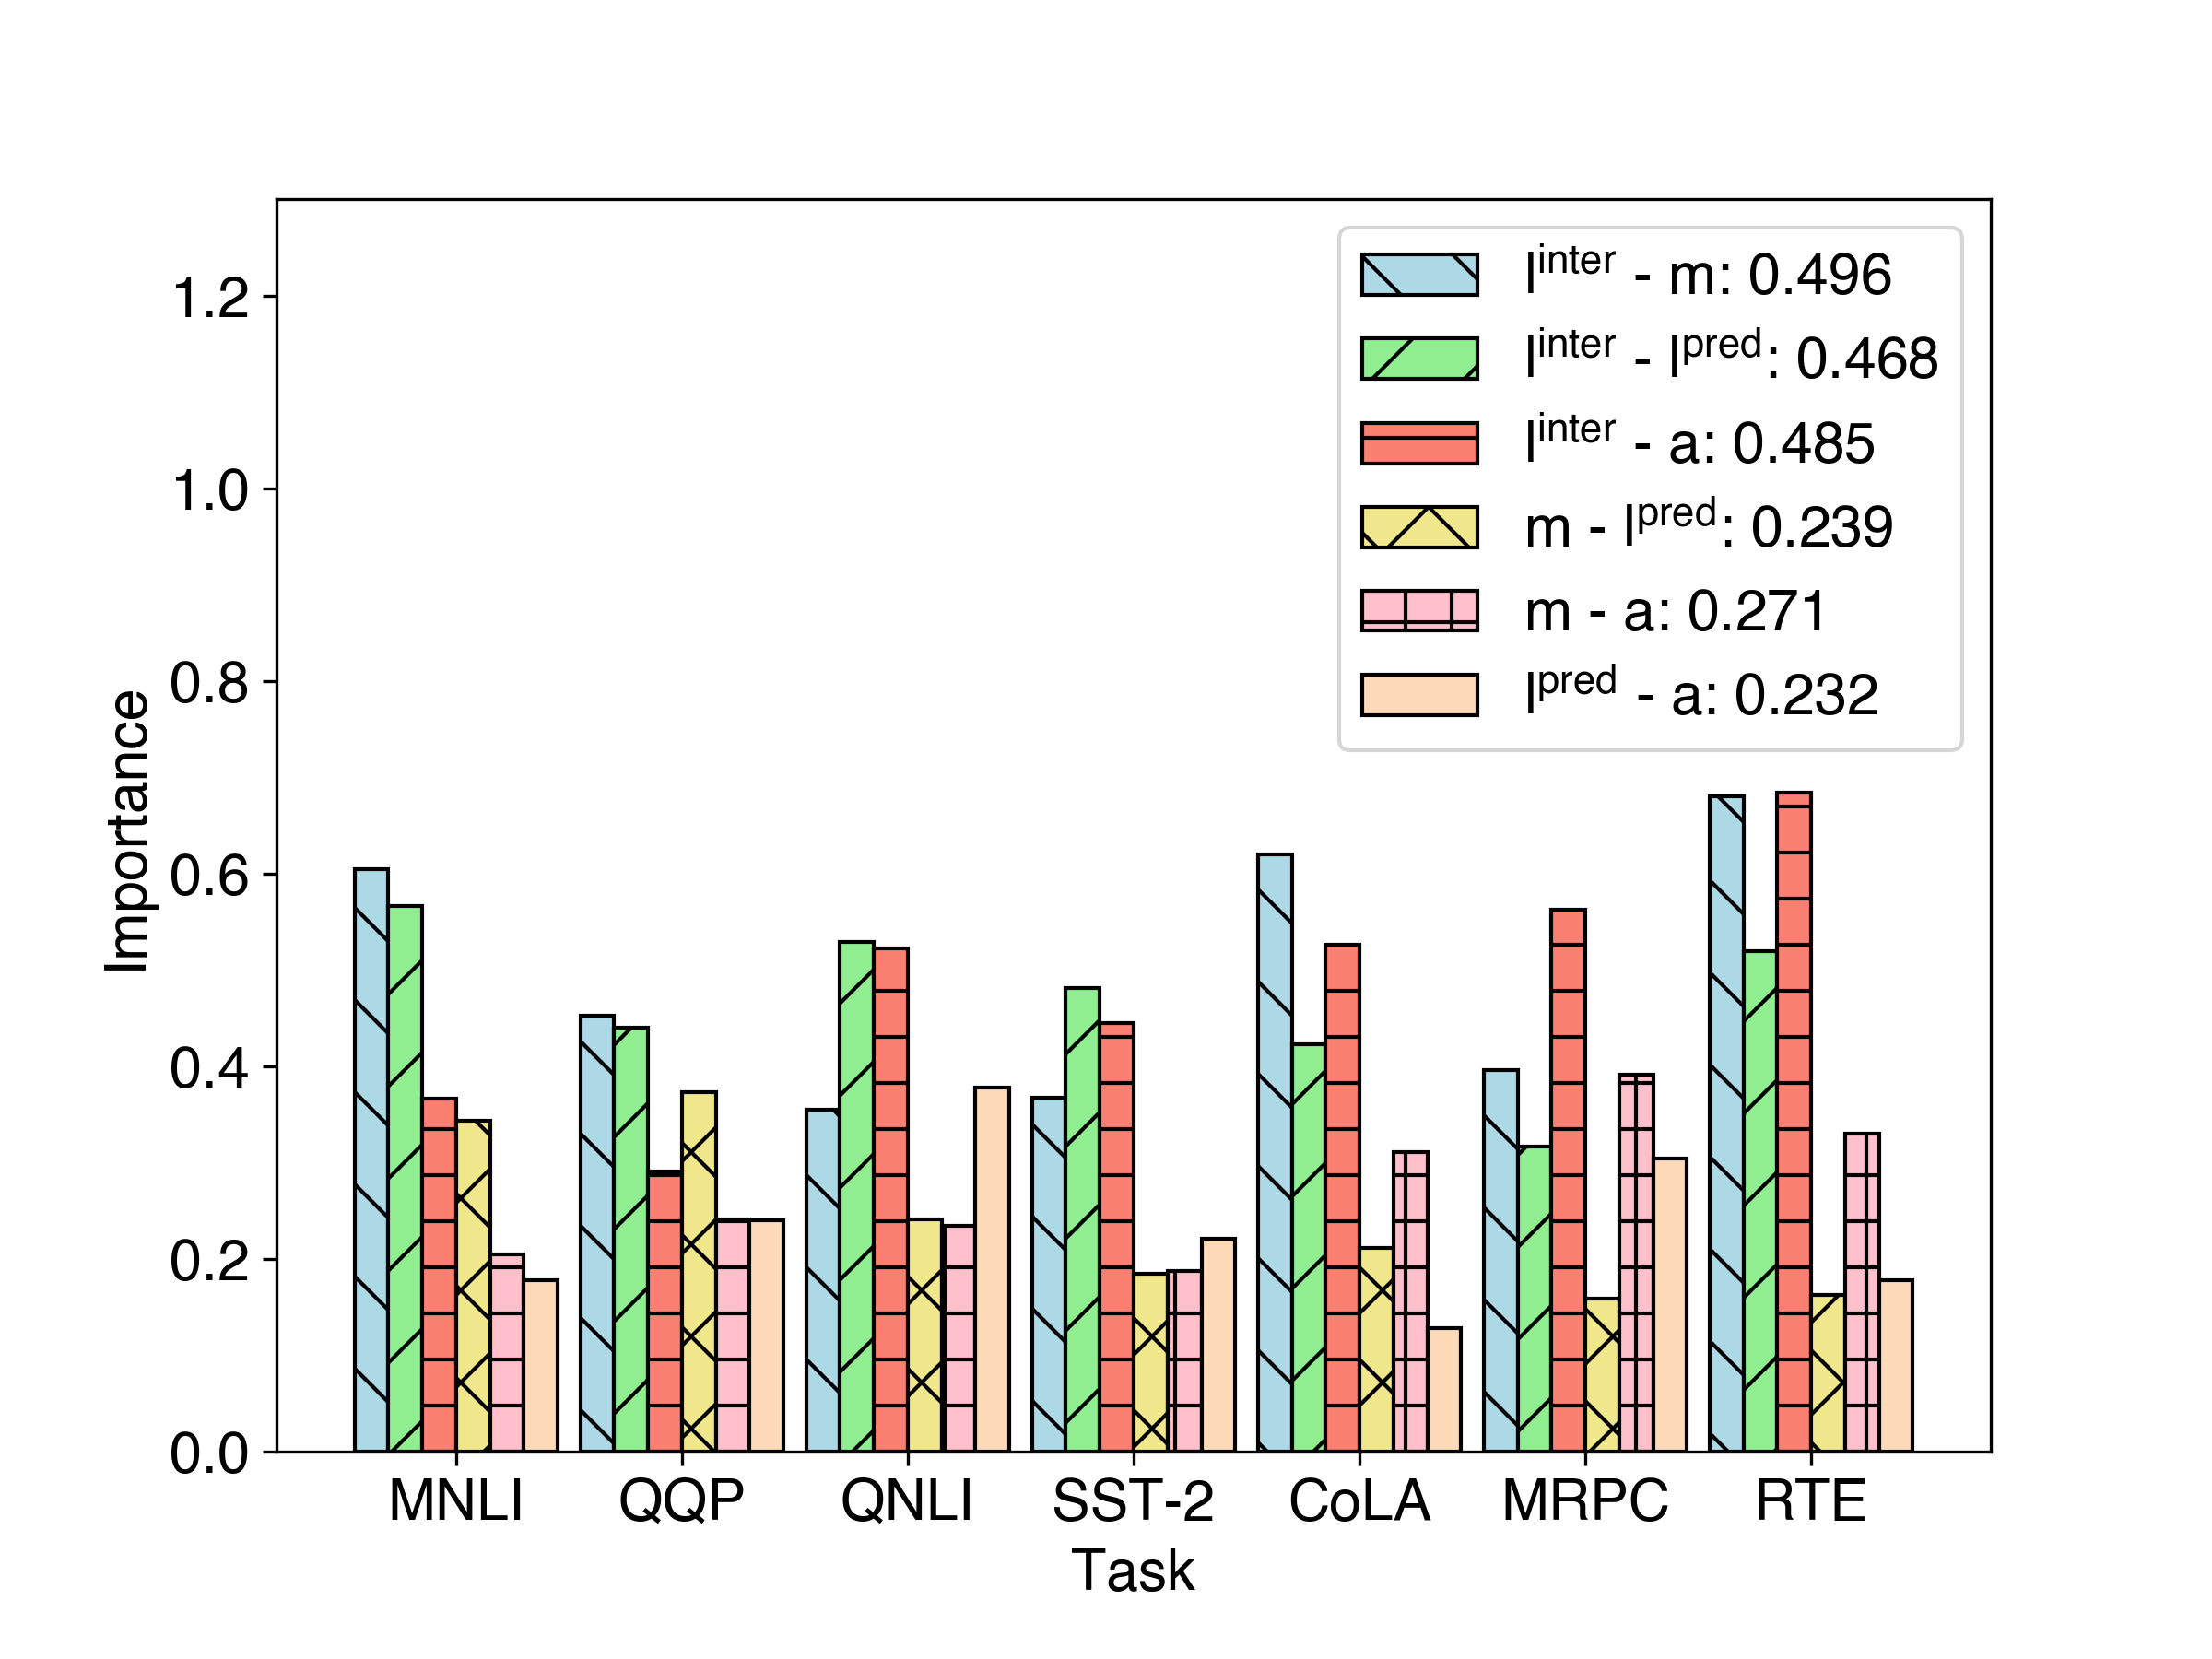
\includegraphics[width=1.0\textwidth]{pics/fanova_double_wo_stsb.png}
%    \end{minipage}
    \caption{}
    \end{subfigure}
    % \vspace{-1em}
    \caption{As assessed via fANOVA, we report the individual importance of the four Distiller components in (a) and importance of interactions between any two of the four components in (b). Four components are: $l^{\text{inter}}$ for intermediate distillation objective, $l^{\text{pred}}$ for prediction layer distillation objective, $a$ for data augmentation and $m$ for layer mapping strategy. Average importance for each component (across tasks) is listed in the legend.}
    \label{fig:fanova}
    \vspace{-1em}
\end{figure*}


\subsection{Performance of AutoDistiller}


Recall that in Section \ref{sec:autodistiller}, we construct the performance prediction model \emph{AutoDistiller} on the extracted dataset features and previously collected experimental results (over 1300 pieces). Here we split all experimental results in a (80/20) train/test ratio then train and evaluate \emph{AutoDistiller} via AutoGluon-Tabular~\citep{erickson2020autogluon}, a simple AutoML tool for supervised learning. 

As we construct dataset features from scratch, it is essential to evaluate how much these features contribute to the final performance of \emph{AutoDistiller}. Therefore, we compute permutation feature importance \citep{breiman2001random}, which is defined as the drop of prediction accuracy after the values of a particular feature are shuffled in the test data. From the results in Figure \ref{fig:permutation} in Appendix, we observe that all features pertain positive importance, among which the task and context embeddings are the two features with the highest feature importance. This shows that the dataset domain and problem type are important factors to consider when constructing AutoDistiller features.

Given that the objective of \emph{AutoDistiller} is to recommend near optimal distillation configurations for new datasets, we applied \emph{AutoDistiller} on two datasets ``BoolQ''~\citep{wang2019superglue} and ``cloth''~\citep{shi2021multimodal} that are not considered in our previous experiments to evaluate its adaptability. In Section \ref{sec:autodistiller}, we discussed that \emph{AutoDistiller} can be continuously updated with more distillation results due to the carefully designed scheme. Here we conducted an ablation experiment to verify the necessity of having more datasets for training \emph{AutoDistiller}. We gradually increase the number of datasets for training \emph{AutoDistiller} and compare the performance of the students trained under the recommended distillation configurations. Results in Figure~\ref{fig:AD:more-data} demonstrate that scaling of AD training data produces more stable distillation strategies.
In addition, we evaluate the effectiveness of \emph{AutoDistiller} by comparing the distillation ratios obtained by the top-$N$ strategies suggested by \emph{AutoDistiller} with the distillation ratios from $N$ randomly sampled strategies. Results are shown in Figure~\ref{fig:AD:compare-random}. We observe that both groups of randomly selected strategies experience high variance in performance and may even be worse than a finetuned student from scratch (distillation ratio $<0$). Randomly combining techniques in different components to form a KD strategy performs as a lottery ticket, which is inefficient in practical AutoML cases. We see great potential that a tool as AutoDistiller can solve this issue as a result of the stable and effective KD strategies it recommends. 
% The best strategy suggested by \emph{AutoDistiller} achieves an accuracy of $75.0$ on ``BoolQ'' and $70.1$ on ``cloth'', close or superior to the teacher performance ($74.0$ on ``BoolQ'' and $71.2$ on ``cloth'').

% can find that distillation pipelines recommened by \emph{AutoDistiller} significantly outperforms randomly sampled pipelines. 
% The random selection rule is: randomly sample N configurations from Distiller search space and keep the configuration with best prediction.
\begin{figure}[!tb]
    \centering
    \begin{subfigure}[b]{0.4\textwidth}
    \centering
    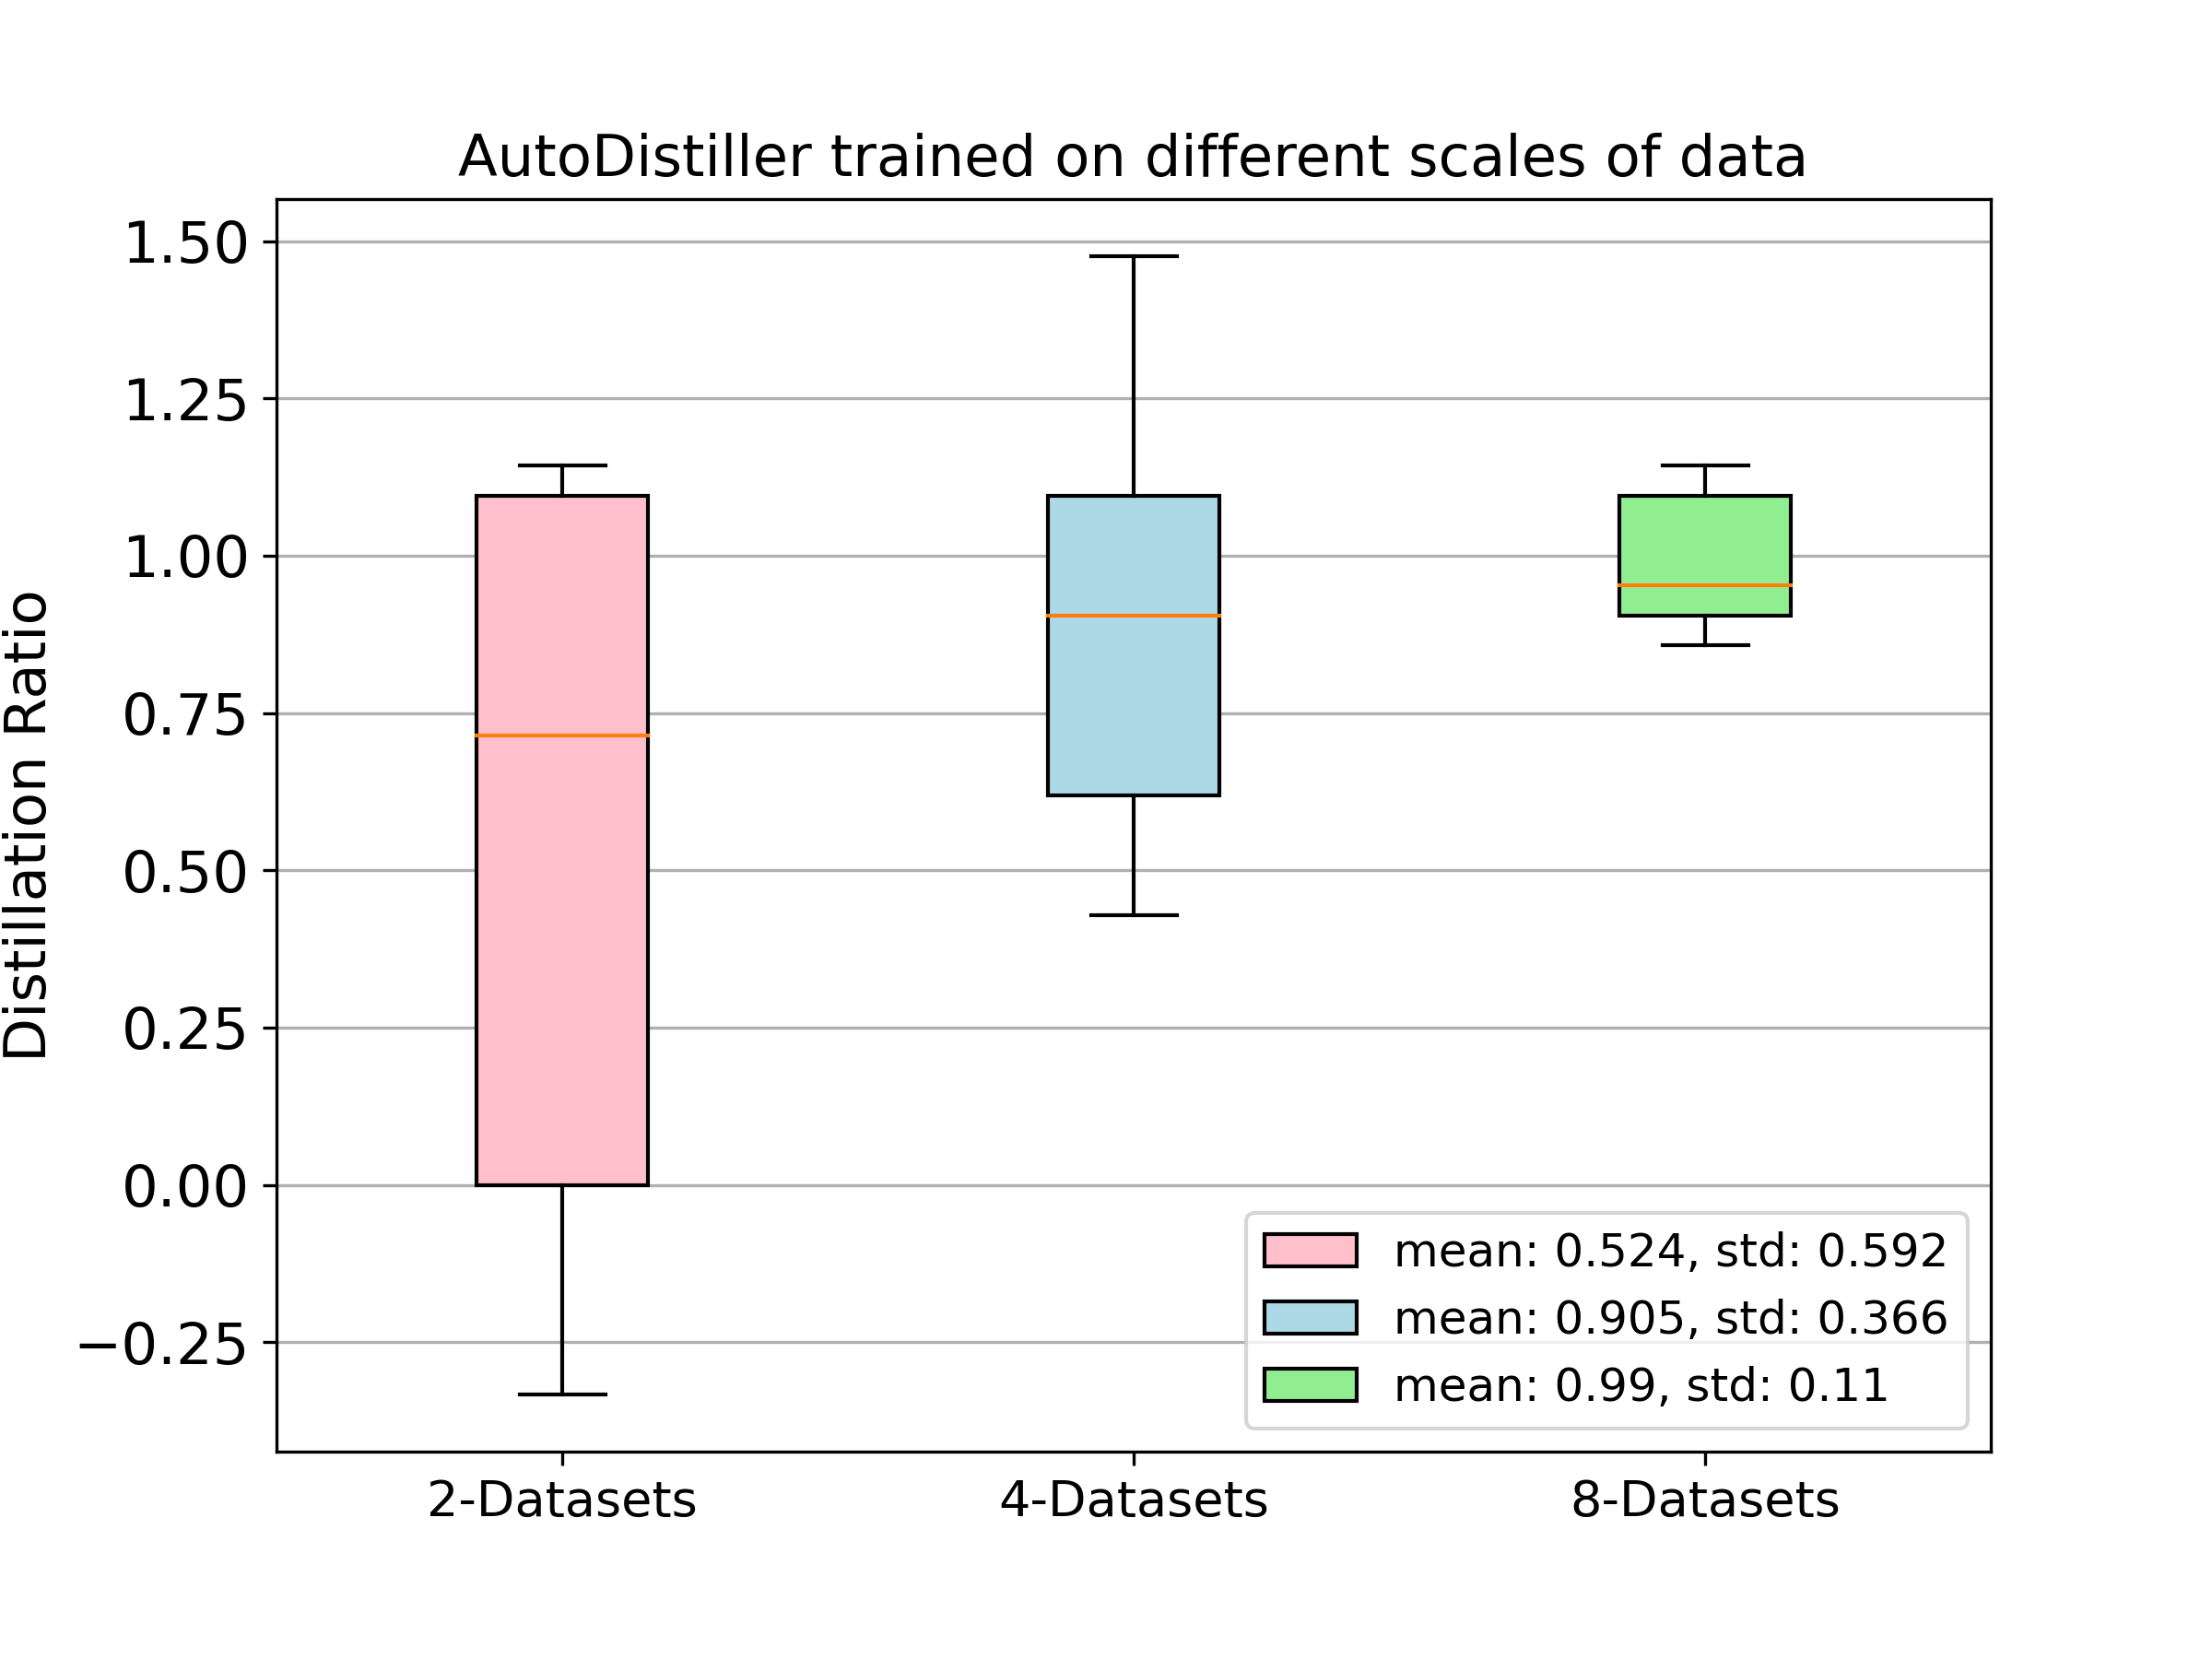
\includegraphics[width=1.0\textwidth]{pics/autodistiller_xscale_scracth.png}
    \caption{AD trained on results of 2, 4, 8 tasks. The scaling of AD training data avoid producing trivial strategies where distillation is worse than finetuning.
    %Though the best strategy is found by 4-Dataset AD, 
    %in general.
    }
    \label{fig:AD:more-data}
    \end{subfigure}
    \begin{subfigure}[b]{0.40\textwidth}
%    \begin{minipage}{6cm}
    \centering
    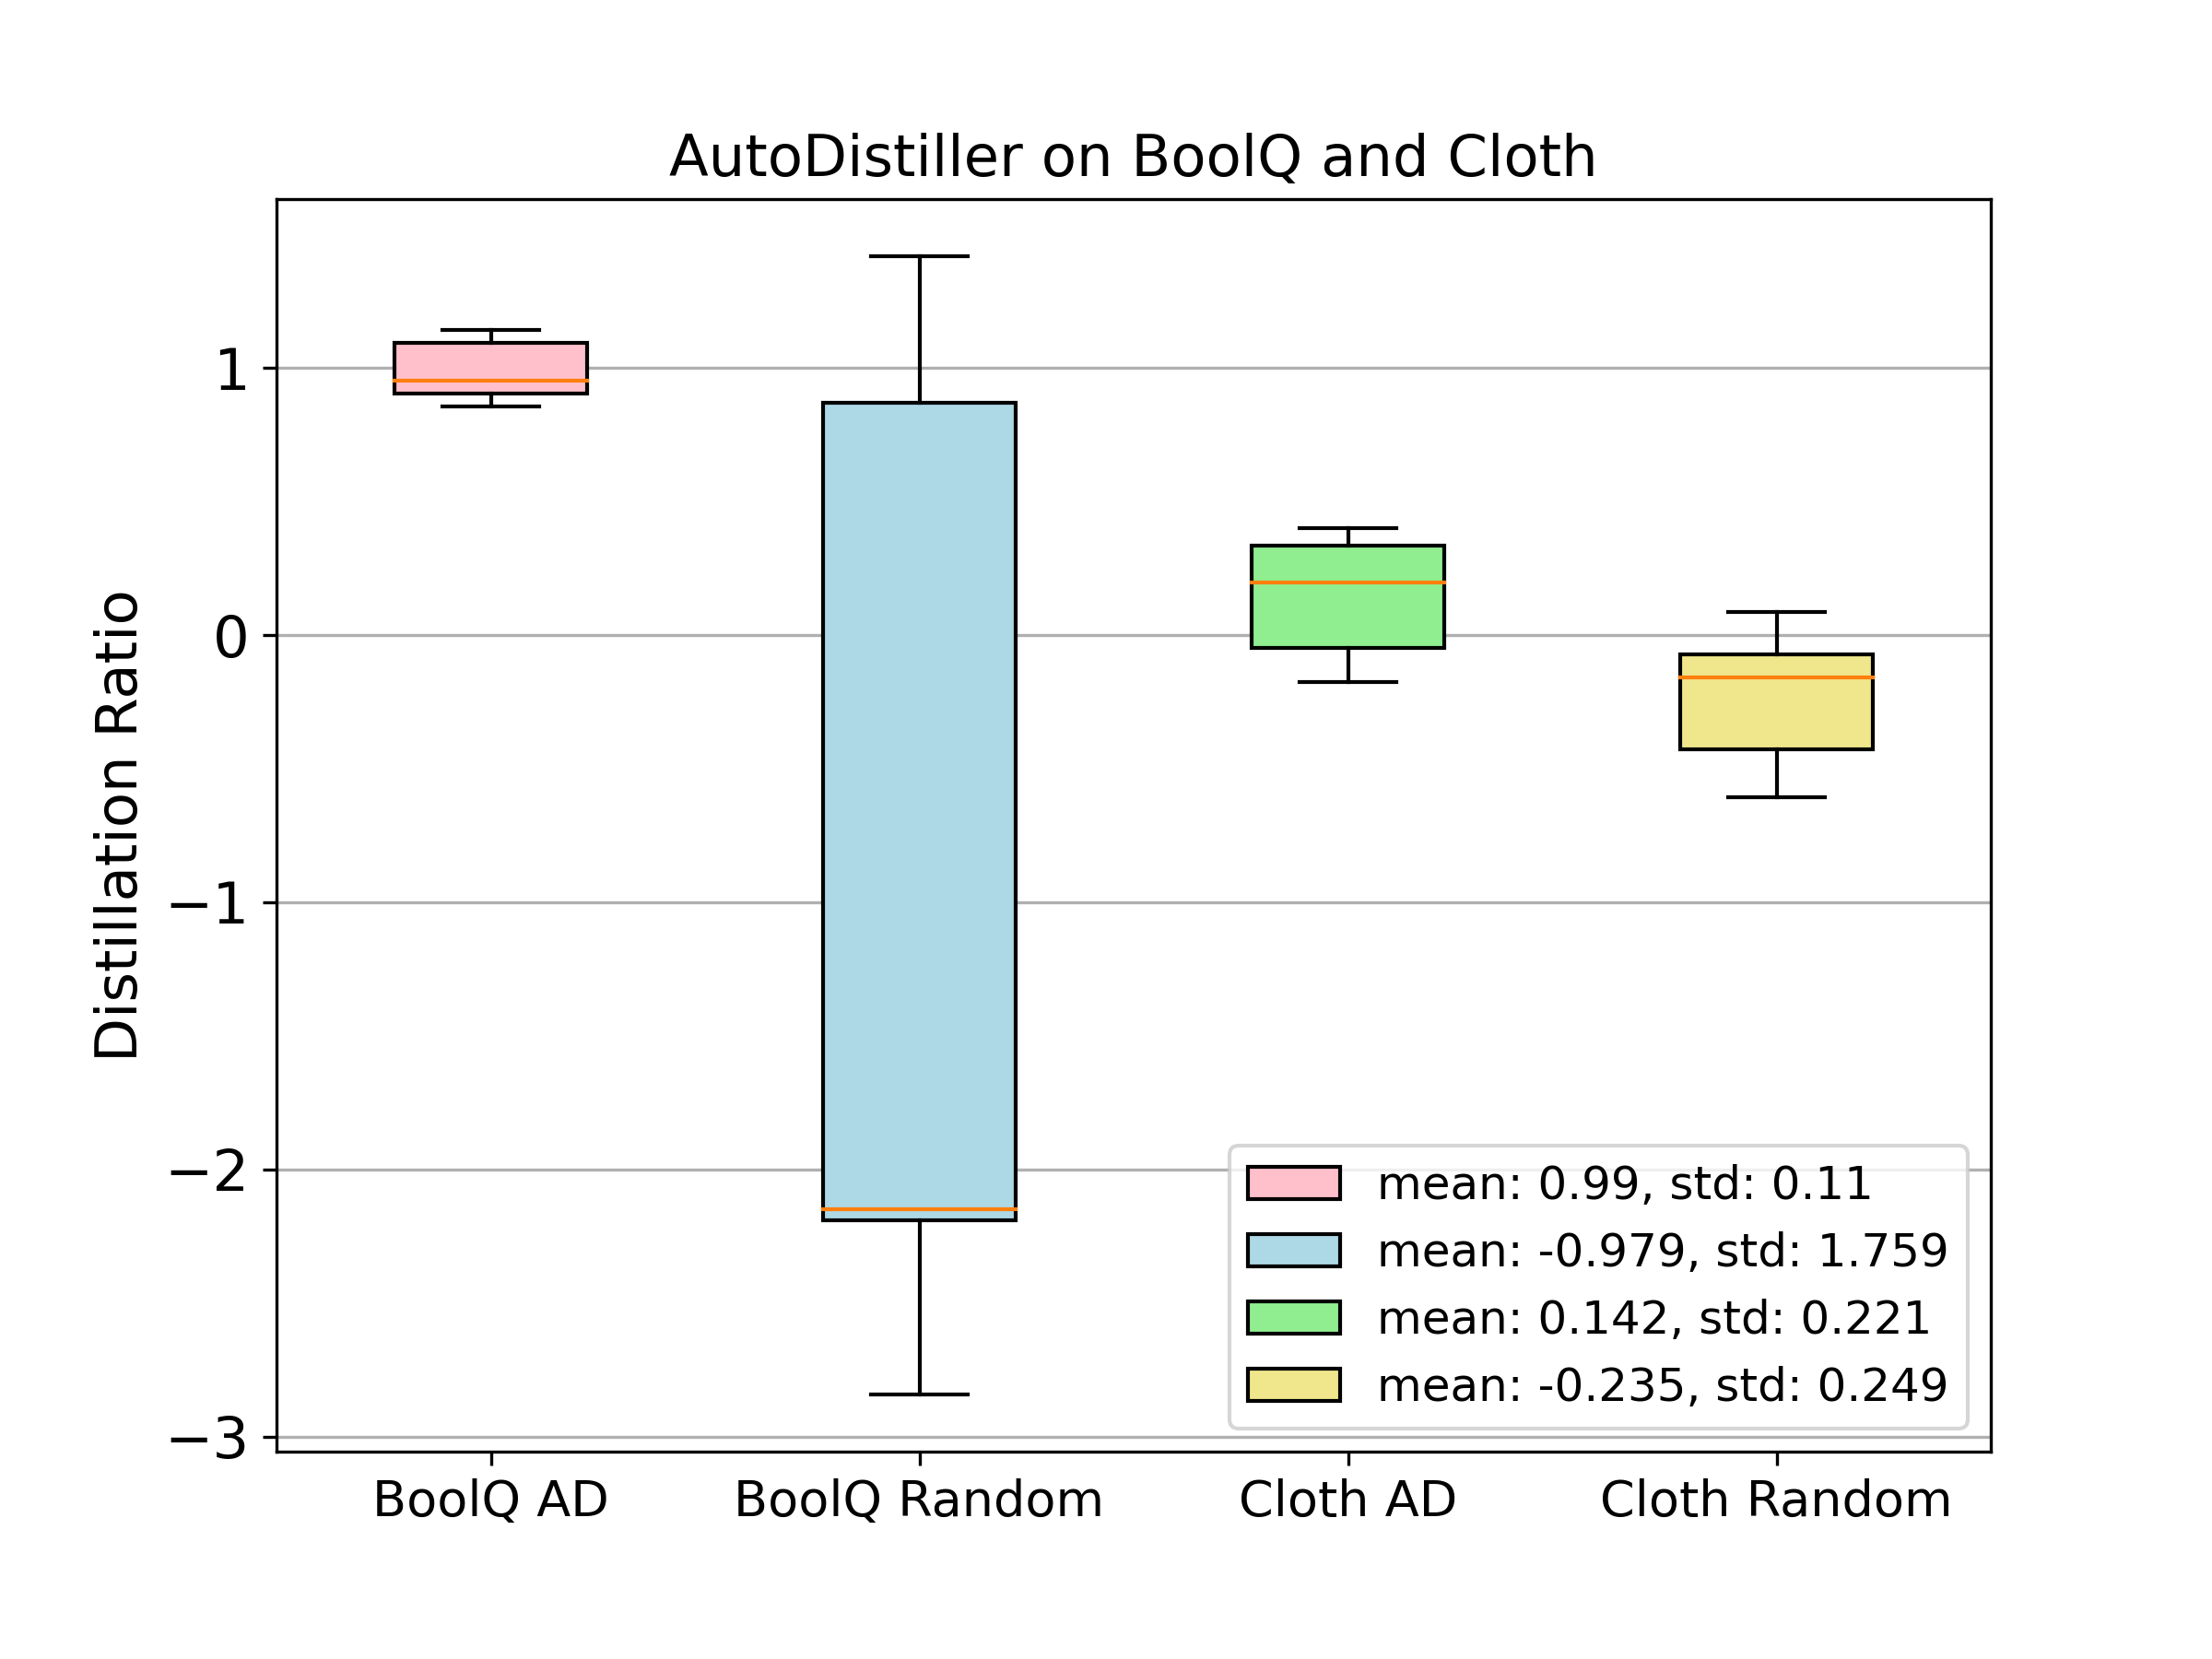
\includegraphics[width=1.0\textwidth]{pics/AD_prediction_scracth.png}
%    \end{minipage}
    \caption{Top-5 AD strategies vs.\ 5 randomly selected strategies. AD significantly outperforms random search on both tasks.}
    \label{fig:AD:compare-random}
    \end{subfigure}
    \caption{Distillation ratio of  \emph{AutoDistiller} (AD) recommended strategies given teacher $\text{BERT}_\text{BASE}$ and student $\text{TinyBERT}_4$ under two settings. Higher ratio indicates better distillation performance. Mean and standard deviation of the groups of ratios are listed in the legend.}
    \label{fig:AD}
    \vspace{-1em}
\end{figure}


\section{Discussion}
\label{discussion}

Large amount of KD algorithms are under a tendency to optimize separate components in the entire KD pipeline, complicating the search space of distillation techniques that are applied on different benchmarks, which fails to match industry demand to automatically select the best distillation strategy for heterogeneous downstream tasks. 
% This calls for a better understanding of existing KD techniques and a self-adaptive scheduler to decide KD strategy for various downstream tasks. 
Our work makes efforts to approach this by proposing an automated distillation system \emph{AutoDistiller} and experimental results reveal the promising vision of a stable and evolvable automated KD system.

Since automated distillation is fairly a new concept, this work aims to put forth a \emph{proof-of-concept} and seeks to answer research questions instead of making a `\emph{sotaeesque}' comparison. We leave extensive comparisons on other setups and baselines to future work. Because \emph{AutoDistiller} serves as a baseline solution to automated KD, it has several limitations: 1) \emph{AutoDistiller} lacks of training data because the 1300+ data points we collect from our experimental results are not a formally constructed dataset but products of meta-learning,  and 2) \emph{AutoDistiller} is compared only to randomly selected strategies, which is a low bar given the complex KD pipeline. We hope that as the \emph{AutoDistiller} shows its potential, automated KD will become a research area that bridges academic research and industry demands. 


\newpage

\clearpage
\bibliography{references}
% and for biber / biblatex, use:

% \printbibliography
\newpage
% supplemental material -- everything hereafter will be suppressed during
% submission time if the hidesupplement option is provided!
\appendix
% \twocolumn[
% \begin{center}
% {\Large \textbf{Appendix -- \  
% Distiller: A Systematic Study of Knowledge Distillation Methods \\ \hspace*{-33mm}  in Natural Language Processing}}
% \vspace*{2em}
% \end{center}
% ]
\begin{center}
{\Large \textbf{Appendix. -- Towards Automated Distillation: A Systematic Study of Knowledge Distillation in Natural Language Processing}}    
\end{center}
% \section{Appendix. -- Towards Automated Distillation: A Systematic Study of Knowledge Distillation in Natural Language Processing}

\section{Distiller}
\label{sec:distiller}
\subsection{Data Augmentation Policy}
\label{subsec:DA}
\SetKwInput{KwInitial}{Initialize}
\SetKwInput{KwParam}{Params}
\SetKwInput{KwIn}{Input}
\SetKwInput{KwOut}{Output}
\begin{algorithm}[b!]
\scriptsize
  \KwParam{A sequence of elementary data augmentation operations $\mathcal{G}$,
  $\forall \mathcal{G}_j \in \{\textit{CA}, \textit{RA}, \textit{BT},\textit{Mixup} \}$. }
%   \KwParam{$p_t$: the threshold probability; \\$n_k$: top k score tokens will be used for augmentation, only for $\textit{Contextual}$; $\lambda$: mixup ratio for $\textit{Mixup}$ augmentation}
  \KwIn{Training Dataset $\mathcal{D}_{\text{train}}$}
  \KwOut{Augmented dataset $\mathcal{D}_\text{synthesize}$}
  \BlankLine
  Initialize $\mathcal{D}_\text{synthesize} \leftarrow \{\}$ \\
    \ForEach {$\{x_i,y_i\} \in \mathcal{D}_{\text{train}} $}{
    \For{j $\leftarrow$ \text{1 to len}($\mathcal{G}$)}{
        $\hat{x}_i,\hat{y}_i=\mathcal{G}_j(x_i,y_i)$\;
        $x_i, y_i \leftarrow \hat{x}_i,\hat{y}_i $\;
     } 
    $\mathcal{D}_\text{synthesize}\leftarrow \mathcal{D}_\text{synthesize}\cup \{x_i,y_i\}$
    }
  \caption{Data Augmentation Policy}
  \label{algo:augmentation_alg}
\end{algorithm}
% In KD, training a student to achieve near performance to the teacher can be a tough task, especially when the teacher is much stronger than the student. 
When the amount of labeled data is small, data scarcity becomes a key challenge for training students.
This can be mitigated via Data Augmentation~(DA) by generating additional data samples. Unlike in supervised learning, where labels for synthetic augmented data may be unclear unless the augmentation is limited to truly benign perturbations, the soft labels for augmented data in KD are simply provided by the teacher which allows for more aggressive augmentation \citep{fakoor2020fast}. 
% opportunity for student to learn from a stronger teacher. 
Denote the set of training samples of the downstream task as $\mathcal{D}_{\text{train}}$, any augmenter $a(\cdot, \cdot)$ stretches the distribution from $E_{x,y\sim {\mathcal{D}_{\text{train}}}}$ to $E_{\hat{x},\hat{y}\sim {a(x,y)},x,y\sim {\mathcal{D}_{\text{train}}}}$. We consider various elementary DA operations including: 1) MLM-based contextual augmentation (CA) , 2) random augmentation (RA), 3) backtranslation (BT) and 4) mixup. The search space of possible augmentations in \emph{Distiller} is constructed by stacking these four elementary operations in an arbitrary order, as detailed in Algorithm~\ref{algo:augmentation_alg}.
% This can produce augmented sentences that have similar semantic meaning but very different structure. 
% In our implementation, we translate from English to German and then translate German to English.
%In our implementation since we focus on English datasets, we implement English to German and translate 

Mixup constructs a synthetic training example via the weighted average of two samples (including the labels) drawn at random from the training data. To use it in NLP, 
\cite{guo2019augmenting,liang2020mixkd} applied mixup on the word embeddings at each sentence position $x_{i,t}$ with $\lambda \in [0,1]$ as the mixing-ratio for a particular pair of examples $x_i, x_j$:
\begin{equation}
    \hat{x}_{i,t}=\lambda x_{i,t} + (1-\lambda) x_{j,t},~ \hat{y}_i=\lambda y_i + (1-\lambda) y_j,
\end{equation}
Here $\lambda$ is typically randomly drawn from a \textit{Uniform} or \textit{Beta} distribution for each pair, $y_i,y_j$ are labels in one-hot vector format, and $(\hat{x}_{i},\hat{y}_i)$ denotes the new augmented sample. To further extend mixup for sentence tagging tasks, in which each token has its own label, we propose calculating the weighted combination of the ground-truth target at each location $t$ as the new target: 
\begin{equation}
    \hat{x}_{i,t}=\lambda x_{i,t} + (1-\lambda) x_{j,t}, ~ \hat{y}_{i,t}=\lambda y_{i,t} + (1-\lambda) y_{j,t},\
\end{equation}
% Here $y_{i,t}$ is the probability distribution for position $t$ to be selected as start or end position of the answer span. 
Fundamental settings of the other three DA operations can be found in Appendix.
\subsection{Prediction Layer Distillation}
In traditional KD, the student network learns from the output logits of the teacher network, adopting these as soft labels for the student's training data \citep{hinton2015distilling}.  
Here we penalize the discrepancy between the outputs of student vs.\ teacher via:
\begin{equation}
    \mathcal{L}_{\text{pred}}=l^{\text{pred}}(f^T(x), f^S(x)),
\end{equation}
where $l^{\text{pred}}(\cdot,\cdot)$ is the KD loss component whose search space in this work includes either: softmax Cross-Entropy (CE) or Mean Squared Error (MSE).

\subsection{Intermediate Representation Distillation}
To ensure the knowledge is sufficiently transferred, we can allow the student to learn from the intermediate layers of the teacher rather than only the latter's output predictions by minimizing the discrepancies between selected layers from the teacher and the student.
% \JM{add intermediate distillation citations here}.
These high-dimensional intermediate layer representations constitute a much richer information-dense signal than is available in the low-dimensional predictions from the output layer. \citep{sun2019patient} shows that this intermediate distillation scheme enables the student to \emph{patiently} learn the rich information in the teacher's hidden layers. As teacher and student usually have different number of layers and hidden-state dimensionalities, it is not clear how to map teacher layers to student layers and how to measure the discrepancy between their hidden states. Previous works proposed various discrepancy measures for intermediate distillation, including:  Cross-Entropy (CE), Mean Squared Error (MSE), L2 distance, Cosine Similarity (CS), and  Patient Knowledge Distillation (PKD)~\citep{sun2019patient}.
For these objectives, we establish the following result. Proof is in  Appendix \ref{sec:appdx:proof}.
% Based on the recent advancement of Mutual Information (MI) estimation, we proved that optimizing the aforementioned loss functions can be viewed as maximizing different lower bounds of MI, as described in the following theorem.

\begin{theorem}
Minimizing MSE, L2, or PKD loss, and maximizing CS between two random variables $X,Y$ are equivalent to maximizing particular lower bounds of the mutual information $I(X;Y)$. 
\label{theorem:unify}
\end{theorem} 
% The proof of Theorem~\ref{theorem:unify} is relegated to the Appendix. 
In our KD setting, $X$ and $Y$ correspond to the hidden state representations of the student and teacher model (for random training examples), respectively. 
Inspired by this theorem, it is reasonable to use the bounds of MI as intermediate objective functions in KD. 
Particularly, we consider the multisample MI lower bound of  \citep{poole2019variational}, which estimates $I(X;Y)$ given the sample $x, y$ from $p(x, y)$ and another $K$ additional IID samples $z_{1:{K}}$ that are drawn from a distribution independent from $X, Y$:

\begin{footnotesize}
\centering
\begin{align*}
    I(X&;Y) \geq E_{p(x, z_{1:{K}})p(y|x)} \left[\log \frac{e^{f(x,y)}}{\alpha m (y;x, z_{1:{K}})+(1-\alpha)q(y)} \right] - E_{p(x, z_{1:{K}})p(y)} \left[\log \frac{e^{f(x,y)}}{\alpha m (y;x, z_{1:{K}})+(1-\alpha)q(y)} \right] + 1 \triangleq I_{\alpha}.     \numberthis
\end{align*}
\end{footnotesize}
% \JM{$X_{2:K}$ seems to be missing from this formula and should be discussed more. Also would be good to use $Z$ instead of $X_2$, so that way you don't need to introduce the weird notation $X_1$ and can just use $X$ instead.}


In $I_\alpha$, $f(\cdot,\cdot)$ and $q(\cdot)$ are critic functions for approximating unknown densities  and $m(\cdot,\cdot)$ is a Monte-Carlo estimate of the partition function that appears in MI calculations. Typically, the space $z$ and the sample $x,y$ are from the same mini-batch while training, namely the mini-batch size is $K+1$. $I_\alpha \in [0, 1]$ flexibly trade off bias and variance, since increasing $\alpha$ reduces the variance of the estimator while increasing its bias. We propose to use $I_\alpha$ as an objective for intermediate distillation and call it MI-$\alpha$. Our implementation leverages a Transformer encoder~\citep{vaswani2017attention} to learn $f(\cdot,\cdot)$ and $q(\cdot)$. To our knowledge, this is the first attempt to utilize complex neural network architectures for critic functions in MI estimation; typically only shallow multi-layer perceptrons (MLPs) are used~\citep{tschannen2019mutual}. Our results in Table \ref{tab:MI-critics} reveal that Transformer produces a better critic function than MLP.

Note that for intermediate distillation, objectives like MSE attempt to ensure the teacher and student representations take matching values, whereas objectives like MI (and tighter bounds thereof) merely attempt to ensure the information in the teacher representation is also captured in the student representation. 
The latter aim is conceptually better suited for KD, particularly in settings where the student's architecture differs from the teacher, in which case forcing intermediate student representations to take the same values as teacher representations may even be harmful for tiny student networks that lack the capacity to learn the same function composition used by the teacher. Besides, MSE in theory measures two variables with matched size, while MI-$\alpha$ is more flexible in variable size due to the use of neural critic functions. This feature of MI-$\alpha$ makes it particularly suitable for KD, where the intermediate representations of the student and the teacher may differ in dimensions.
We emphasize that a high MI between student and teacher representations suffices for the teacher's prediction to be approximately recovered from the student's intermediate representation (assuming the teacher uses deterministic output layers as is standard in today's NLP models). Given that high MI suffices for the student to match the teacher, we expect tighter MI bounds like MI-$\alpha$ can outperform looser bounds like MSE that impose additional requirements on the student's intermediate representations beyond just their information content.
\subsubsection{Layer Mapping Strategy}
We investigate three intermediate layer mapping strategies: 1) Skip: the student learns from every $\floor{M/N}$ layer of the
% \todo{denote layer mapping strategy with $m_{i,j}$ or a function $n=g(m)$}
teacher, i.e., $m_{i,j}=1$ when $j=i\times \floor{M/N}$; 2) Last: the student learns from the last $k$ layers of the teacher, i.e., $m_{i,j}=1$ when $j=i+M - N$; and 3) EMD: a many-to-many learned layer mapping strategy~\citep{li2020bert} based on Earth Mover's Distance. The intermediate loss with EMD mapping can be denoted as:

\begin{equation}
    \mathcal{L}_{\text{EMD}}(H^S_{1:N},H^T_{1:M})=\frac{\sum_{i=1}^{M}\sum_{j=1}^{N}w_{i,j}^H d_{i,j}^H}{\sum_{i=1}^{M}\sum_{j=1}^{N}w_{i,j}^H},
\end{equation}
where $D^H=[d_{i,j}^H]$ is a distance matrix representing the cost of transferring the hidden states knowledge from $H^T$ to $H^S$. And $W^H=[w_{i,j}^H]$ is the mapping flow matrix which is learned by minimizing the cumulative cost required to transfer knowledge from $H^T$ to $H^S$. In \emph{Distiller}, the distance matrix is calculated via intermediate objective function: $d_{i,j}^H=l^{\text{inter}}(H_i^S,H_j^T)$.  

\section{Proof of Theorem \ref{theorem:unify}}
\setcounter{theorem}{0}
\renewcommand{\theequation}{A.\arabic{theorem}}
% \subsection{Proof of Theorem 1}
\label{sec:appdx:proof}
\noindent Denote the Mutual Information (MI) between two random variables $X$ and $Y$ as $I(X; Y)$. Based on the results on variational bounds of MI~\citep{poole2019variational}, we derive a theorem that optimizing common knowledge distillation objectives, including Mean Squared Error (MSE), L2 distance, and cosine similarity between $X$ and $Y$, can be viewed as maximizing certain lower bounds of $I(X; Y)$. To prove the theroem, we leverage this lemma:

\begin{lemma}
[$I_{\text{TUBA}}$]
Assume that $f(x,y)$ is an arbitrary neural network that takes $x$ and $y$ as inputs and outputs a scalar and $a(y)>0$. The lower bound of $x$ and $y$ can be estimated by:
\begin{small}
\begin{equation*}
\begin{aligned}
    I (X;Y) &\geq E_{p(x,y)}[ \log \frac{e^{f(x,y)}}{a(y)}] - E_{p(x)p(y)}[\frac{e^{f(x,y)}}{a(y)}] \triangleq I_{\text{TUBA}}.
\end{aligned}
\end{equation*}
\end{small}
\label{lemma:tuba}
\end{lemma}

% \subsection*{Lemma 1 ($I_{\text{TUBA}}$)}
% Assume that $f(x,y)$ is an arbitrary neural network that takes $x$ and $y$ as inputs and outputs a scalar and $a(y)>0$. We have:
% \begin{scriptsize}
% \begin{equation}
%     I (X;Y) \geq E_{p(x,y)}[ \log \frac{e^{f(x,y)}}{a(y)}] - E_{p(x)p(y)}[\frac{e^{f(x,y)}}{a(y)}] \triangleq I_{TUBA}
% \end{equation}
% \end{scriptsize}

% \noindent\emph{Proof.}
\begin{proof}
Based on the definition of MI, we have:
\begin{equation*}
    \begin{aligned}
        I(X;Y)&=E_{p(x,y)}[\log\frac{p(x|y)}{p(x)}] =E_{p(x,y)}[\log \frac{p(y|x)}{p(y)}].
    \end{aligned}
\end{equation*}
  Replacing the intractable conditional distribution $p(x|y)$ with a tractable variational distribution $q(x|y)$ yields a lower bound on MI due to the non-negativity of the KL divergence:
\begin{equation*}
    \begin{small}
\begin{align}
\label{eq:tuba-proof-main}
        I(X;Y)&=E_{p(x,y)}[\log \frac{q(x|y)}{p(x)}]+E_{p(x,y)}[\log \frac{p(x|y)}{q(x|y)}] \notag\\
        &=E_{p(x,y)}[\log \frac{q(x|y)}{p(x)}]+E_{p(y)}[KL({p(x|y)}||{q(x|y)})]\\ 
        &\geq E_{p(x,y)}[\log q(x|y)]+H(X) \notag,
\end{align}
\end{small}
\end{equation*}

where $H(X)$ is the entropy of $X$. Then we choose an energy-based variational family that uses a critic function $f(x,y)$ and is scaled by the data density $p(x)$ to represent $q(x|y)$:
\begin{equation*}
    q(x|y)=\frac{p(x)}{Z(y)}e^{f(x,y)} , Z(y)=E_{p(x)}[e^{f(x,y)}].
\end{equation*}
Substituting this distribution into \eqref{eq:tuba-proof-main} gives a lower bound on MI:
\begin{equation*}
    I(X;Y)\geq E_{p(x,y)}[f(x,y)]-E_{p(y)}[\log Z(y)].
\end{equation*}
However, this objective is still intractable. To form a tractable bound, we can upper bound the log partition function by this inequality: $\log(x)\leq \frac{x}{a}+\log(a)-1$ for all $x,a>0$. Apply this inequality to get:
\begin{small}
\begin{equation*}
    \begin{split}
        I(X;Y)&\geq E_{p(x,y)}[f(x,y)]-E_{p(y)}[\log Z(y)]\\ &\geq E_{p(x,y)}[f(x,y)]-E_{p(y)}[\frac{E_{p(x)}[e^{f(x,y)}]}{a(y)}+\log a(y)-1]\\
        &= E_{p(x,y)}[f(x,y)] - E_{p(x,y)}[\log a(y)] \\
        &- E_{p(x)p(y)}[\frac{e^{f(x,y)}}{a(y)}]+1\\
        &\geq E_{p(x,y)}[\log \frac{e^{f(x,y)}}{a(y)}] - E_{p(x)p(y)}[\frac{e^{f(x,y)}}{a(y)}].
    \end{split}
\end{equation*}
\end{small}
This bound holds for any $a(y)>0$.
\end{proof}


\begin{theorem}
Minimizing MSE, L2, or PKD loss, and maximizing the cosine similarity between two random variables $X,Y$ are equivalent to maximizing particular lower bounds of the mutual information $I(X;Y)$. In knowledge distillation, samples $x \in X$ and $y \in Y$ are hidden states generated by the student model and teacher model.
\end{theorem} 

% \subparagraph*{Theorem 1. }\\\\
\begin{proof}
We prove this theorem by constructing $f(x,y)$ and $a(y)$ in Lemma \ref{lemma:tuba} for each loss function. 
\subparagraph{MSE}
$\mathcal{L}_{\text{MSE}}(x,y) = ||x-y||_2^2$, let $f(x,y) = -||x-y||_2^2, a(y)=1$, we have:
\begin{small}
\begin{equation}
\begin{split}
 I (X;Y)&\geq E_{p(x,y)}[\log e^{-||x-y||_2^2}] - E_{p(x)p(y)}[e^{-||x-y||_2^2}] \notag \\
&\geq  E_{p(x,y)}[\log e^{-||x-y||_2^2}] - E_{p(x)p(y)}[e^0]\\ 
&= E_{p(x,y)}[\log e^{-||x-y||_2^2}] - 1\\
&= E_{p(x,y)}[-||x-y||_2^2] - 1.
\end{split}
\end{equation}
\end{small}

Therefore, minimizing the MSE loss between $x$ and $y$ can be viewed as maximizing the lower bound of $I(X;Y)$.
\subparagraph{PKD Loss}
$\mathcal{L}_{\text{PKD}}(x, y) = ||\frac{x}{||x||_2}-\frac{y}{||y||_2}||_2^2$, let $f(x,y)=-||\frac{x}{||x||_2}-\frac{y}{||y||_2}||_2^2$, we have:
\begin{small}
\begin{equation*}
\begin{split}
 I (X;Y)&\geq E_{p(x,y)}[\log e^{-||\frac{x}{||x||_2}-\frac{y}{||y||_2}||_2^2}] \\
 &- E_{p(x)p(y)}[e^{-||\frac{x}{||x||_2}-\frac{y}{||y||_2}||_2^2}] \\
&\geq  E_{p(x,y)}[\log e^{-||\frac{x}{||x||_2}-\frac{y}{||y||_2}||_2^2}] - E_{p(x)p(y)}[e^0] \\ 
&= E_{p(x,y)}[\log e^{-||\frac{x}{||x||_2}-\frac{y}{||y||_2}||_2^2}] - 1\\
&= E_{p(x,y)}[-||\frac{x}{||x||_2}-\frac{y}{||y||_2}||_2^2] - 1 .
\end{split}
\end{equation*}
\end{small}

Consequently, minimizing the PKD loss between $x$ and $y$ can be viewed as maximizing the lower bound of $I(X;Y)$.

\subparagraph{L2 Loss}

$\mathcal{L}_{L_2}(x,y) = ||x-y||_2$, let $f(x,y)=-||x-y||_2$, a(y)=1, we have:
\begin{small}
\begin{equation}
\begin{split}
I (X;Y)&\geq  E_{p(x,y)}[\log e^{-||x-y||_2}] - E_{p(x)p(y)}[e^{-||x-y||_2}] \notag \\
&\geq  E_{p(x,y)}[\log e^{-||x-y||_2}] - E_{p(x)p(y)}[e^0] \notag \\
&= E_{p(x,y)}[\log e^{-||x-y||_2}] - 1\\&= E_{p(x,y)}[-||x-y||_2] - 1 .
\end{split}
\end{equation}
\end{small}

Consequently, minimizing the L2 loss between $x$ and $y$ is equivalent to maximizing the lower bound of $I(X,Y)$.
\subparagraph{Cosine Similarity}
The cosine similarity between two hidden states $x$ and $y$ is calculated as $\frac{x \cdot y}{||x||\times||y||}$, let $f(x,y)=\frac{x \cdot y}{||x||\times||y||}-1, a(y)=1$
\begin{small}
\begin{equation*}
\begin{split}
I(X,Y)&\geq E_{p(x,y)}[\log e^{\frac{x \cdot y}{||x||\times||y||}-1}]-E_{p(x)p(y)}[e^{\frac{x \cdot y}{||x||\times||y||}-1}]\\
&\geq E_{p(x,y)}[\log e^{\frac{x \cdot y}{||x||\times||y||}-1}]-E_{p(x)p(y)}[e^0] \\
&= \frac{1}{e}E_{p(x,y)}[\log e^{\frac{x \cdot y}{||x||\times||y||}}]-1 \\ &= \frac{1}{e}E_{p(x,y)}[\frac{x \cdot y}{||x||\times||y||}]-1 .
\end{split}
\end{equation*}
\end{small}
Consequently, maximizing the cosine similarity between $x$ and $y$ can be viewed as maximizing mutual information between $x$ and $y$.
\end{proof}

\section{Additional Experiment/Computation Details}
\subsection{Distiller Search Space}
\label{sec:app:searchspace}
Here we recap the full search space considered for each stage of the KD pipeline in Distiller:
$l^{\text{inter}}$ $\in$ \{MSE, L2, CS, PKD, MI-$\alpha$ ($\alpha$ = 0.1, 0.5, or 0.9)\}, $l^{\text{pred}}$ $\in$ \{MSE, CE\}, \{$m_{i,j}$\} $\in$ \{Skip, Last, EMD\}, augmentation policy $a$ is one or combinations of elementary augmentation operations in \{CA, RA, BT, Mixup\} .

\subsection{Relationship to Other Distillation Methods}
\label{subsec:distiller_search_space}
\emph{Distiller} is a generic meta-framework that encompasses various KD pipelines used in previous work. For example, Distiller with the following configurations corresponds to the KD pipeline used in each of the cited works: 
$l^{\text{pred}} =$ CE, $l^{\text{inter}}=$ MSE, $m_{i,j} = $ Skip, $a = $ CA  \citep{jiao2019tinybert}; 
$l^{\text{pred}} =$ CE, $l^{\text{inter}}=$ MSE, $m_{i,j} = $ EMD \citep{li2020bert}; 
$l^{\text{pred}} =$ CE, $a = $ Mixup  \citep{liang2020mixkd}.
\subsection{Architecture of Teacher and Student Networks}
\label{sec:app:netarch}
In Table \ref{tab:mi-alpha}, we use two baseline models $\text{BERT-PKD}_4$ and $\text{BERT-EMD}_4$. As described in the original paper \citep{sun2019patient}, we initialize $\text{BERT-PKD}_4$ with the first 4 layers of parameters from pretrained $\text{BERT}_\text{BASE}$. $\text{BERT-EMD}_4$ is initialized from $\text{TinyBERT}_4$ so they have the same architecture.
We list the detailed configurations of the teacher and student architectures investigated in Table \ref{tab:teacher_student_architecture}.
% \begin{figure}[!tb]
%   \centering
%     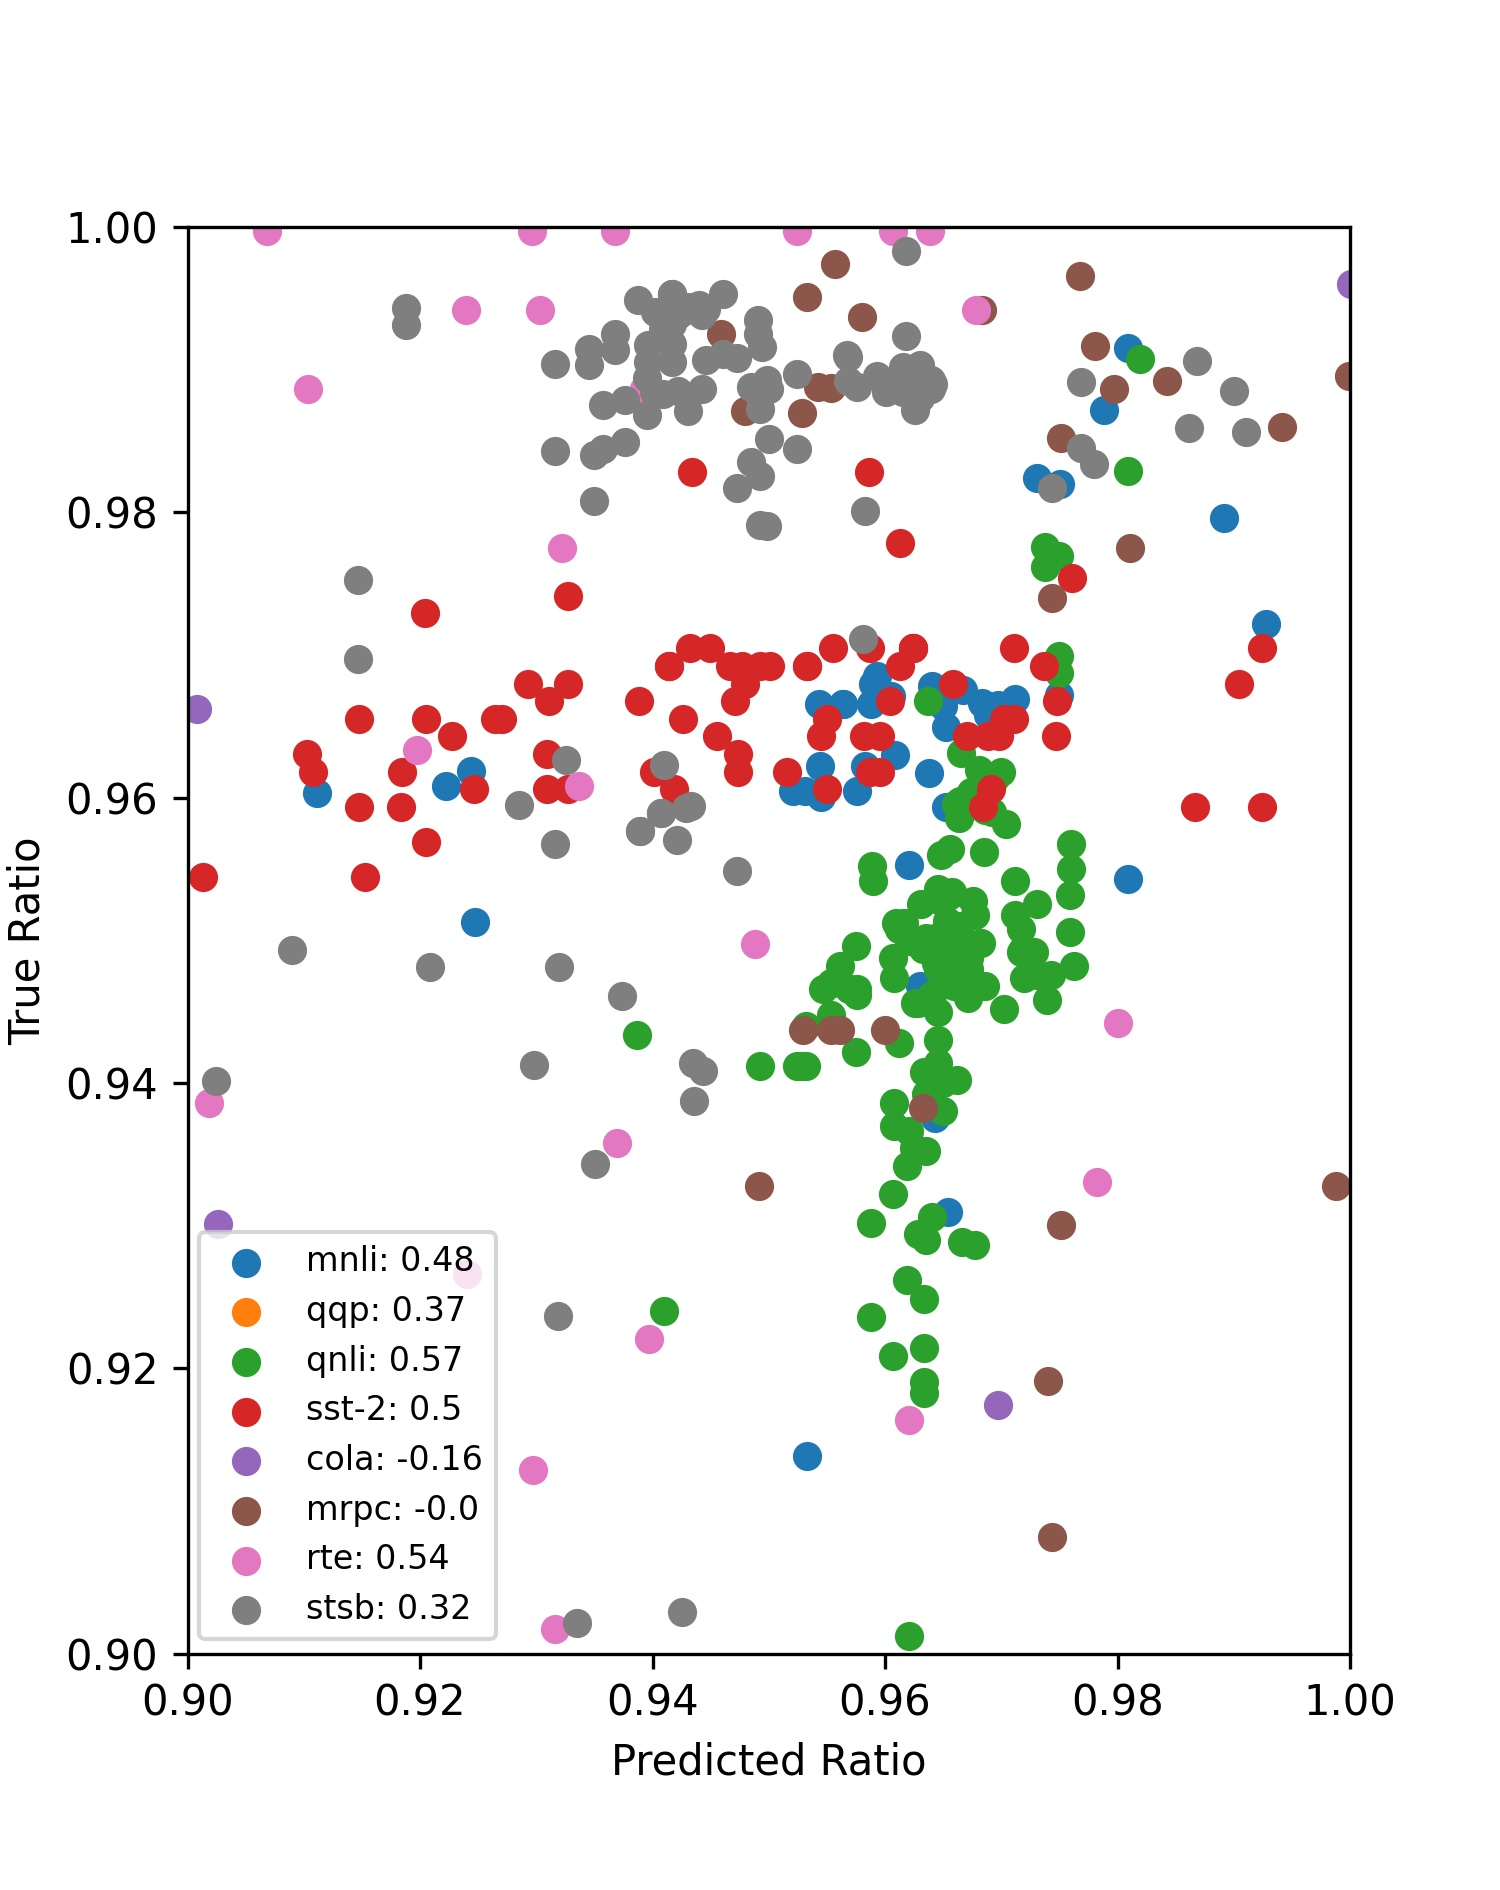
\includegraphics[scale=0.4]{pics/leave_one_out_predictions_100d.jpg}
%   \caption{Evaluating held-out AutoDistiller predictions on GLUE via leave-one-out estimates. We use dataset-level cross-validation that holds out each GLUE dataset from AutoDistiller training. For each held-out dataset, the legend lists Spearman's rank correlation between the predicted vs.\ actual distillation ratio across different KD pipelines. The average Spearman's rank correlation value across the 8 datasets is 0.33.
%   }
% %   \JM{Number in legend needs to be defined. I presume these are some sort of rank correlation, if not, why not report rank correlation somewhere?}
%   \label{fig:leaveoneout}
% \end{figure}
\begin{table}[h]
\centering
\caption{Network architectures of the teacher and student models used in the paper.}
\resizebox{0.6\columnwidth}{!}{%
\begin{tabular}{lccccc}
\toprule
Model & \#Params &  $h_{\text{units}}$ & $n_{\text{layers}}$ & $h_{\text{mid}}$ & $n_{\text{heads}}$ \\
\hline
\multicolumn{6}{c}{Teacher architectures} \\
$\text{RoBERTa}_{\text{LARGE}}$ & 335M & 1024 & 24 & 4096 & 16 \\
$\text{ELECTRA}_{\text{LARGE}}$ & 335M & 1024 & 24 & 4096 & 16 \\
$\text{BERT}_{\text{BASE}}$ & 110M & 768 & 12 & 3072 & 12 \\ \hline
\multicolumn{6}{c}{Student architectures} \\
$\text{TinyBERT}_{\text{6}}$ & 67M & 768 & 6 & 3072 & 12 \\
$\text{BERT-PKD}_4$ & 52M & 768 & 4 & 3072 & 12 \\ 
$\text{BERT}_{\text{MEDIUM}}$ & 41M & 512 & 8 & 2048 & 8 \\
$\text{BERT}_{\text{SMALL}}$ & 29M & 512 & 4 & 2048 & 8 \\
$\text{TinyBERT}_{\text{4}}$ & 14M & 312 & 4 & 1200 & 12 \\
$\text{ELECTRA}_{\text{SMALL}}$ & 14M & 256 & 12 & 1024 & 4 \\
$\text{BERT}_{\text{MINI}}$ & 11M & 256 & 4 & 1024 & 4 \\
$\text{BERT}_{\text{TINY}}$ & 4M & 128 & 2 & 512 & 2 \\
\bottomrule
\end{tabular}
}
\label{tab:teacher_student_architecture}
\end{table}

\subsection{Experimental Setup \& Computing Details}
\label{exps}
% \subsection{Datasets}
% We evaluate \emph{Distiller} on the General Language Understanding Evaluation(GLUE)~\cite{wang2018glue} benchmark which consists of nine sentence-level classification tasks and SQuAD v1.1~\cite{rajpurkar2016squad} which is a span-selection task. The metrics for these tasks can be found in the original papers.
All experiments are evaluated on GLUE~\citep{wang2018glue} and SQuAD v1.1~\citep{rajpurkar2016squad} that contain classification, regression, and tagging tasks. We view SQuAD as a span part-of-speech tagging task by finding the correct answer span from the given context. The same metrics for these tasks as in the original papers~\citep{wang2018glue, rajpurkar2016squad} are adopted.

% \subsection{Distiller Settings}
\citep{turc2019well} finds initializing students with pretrained weights is better for distillation, therefore, we initialize student models with either weights obtained from task-agnostic  distillation~\citep{jiao2019tinybert} or pretrained from scratch~\citep{turc2019well}. Task-specific fine-tuned models $\text{BERT}_\text{BASE}$, $\text{RoBERTa}_\text{LARGE}$, and $\text{ELECTRA}_\text{LARGE}$ are considered as teacher models in our experiments. Models with comparably fewer parameters such as $\text{TinyBERT}_4$, $\text{ELECTRA}_\text{SMALL}$ and others detailed in Table~\ref{tab:teacher_student_architecture} in Appendix are selected as students.
% For evaluating the performance of MI-$\alpha$, we initialize our student model with the 4-layer general distillation model provided by TinyBERT\cite{jiao2019tinybert}, and we finetune BERT model on specific datasets as teacher model. 

For data augmentation, We consider various elementary DA operations including: 1) MLM-based contextual augmentation (CA) , 2) random augmentation (RA), 3) backtranslation (BT) and 4) mixup. For contextual augmentation, we use the pretrained BERT model to do word level replacement by filling in randomly masked tokens. As in EDA  \citep{wei2019eda}, our random augmentation randomly swaps words in the sentence or replaces words with their synonyms. For backtranslation, we translate the sentence from one language (in this paper, English) to another language (in this paper, German) and then translate it back. Unlike existing implementations of DA in NLP that separately generate an augmented dataset first and then recall it over training, in Distiller, we apply a dynamic DA strategy where we generate a new augmented dataset every $U$ ($=5$) epochs during training. We find this strategy to be more time-consuming and flexible as a DA pipeline. In addition, we use the teacher network to compute the soft label $\hat{y}$ assigned to any augmented sample $\hat{x}$.

For hyper-parameters in Equation~\ref{eq:objective}, our preliminary experiments suggest that setting $\beta_1$, $\beta_2$ to $1$ produces the best overall performance so we fix their values to $1$ in subsequent results. $\gamma_1$ and $\gamma_2$ are set to $0.5$ when DA is applied (otherwise $\beta_2$, $\gamma_1$ and $\gamma_2$ are set to $0$). For controlled experiments, unless specified explicitly, we fix ${l^\text{inter}}$ as MI-$\alpha$ $(\alpha=0.9)$ and the layer mapping as ``Skip''. Critic functions in MI-$\alpha$ are powered by a shallow Transformer.  

All experiments are performed on a single machine with 4 NVIDIA T4 GPUs. To reduce the hyper-parameter search space, we fix the batch size as 16 and the learning rate as 5e-5 for all experiments. We used automated mix precision FP16 for training. Maximum sequence length is set to 128 for sentence-pair tasks in GLUE, 64 for single sentence tasks, and 320 for SQuAD. Most of the experiments are trained for 15 epochs except 30 epochs for the challenging task CoLA and 30 epochs for SQuAD. As for the critic functions in MI-$\alpha$, two-layer Transformer($h_\text{mid}=256$, $n_\text{heads}=8$) or 4-layer MLP is the choice in our implementation.
\label{sec:app:com-config}
\begin{table*}[tb!]
\centering
\caption{We extract features from downstream datasets so that every task can be represented as a fixed-dimension embedding. The extracted embedding can be fed into \emph{AutoDistiller} as dense features. In this table, we describe how the embedding is acquired. }
\resizebox{0.8\linewidth}{!}{
\begin{tabular}{l|l}
\toprule
Feature & Description \\ \hline
Context Embedding & \begin{tabular}[c]{@{}l@{}} Every document can be represented as a weighted average of the GloVe vectors,\\ where the weights are defined by the TF-IDF scheme. \\
Each downstream dataset is viewed as a ``document'' in the TF-IDF scheme. \\ Precisely, the embedding of a dataset $s$ is $v_s = \frac{1}{|s|} \sum \limits_{w \in s} \text{IDF}_w \overrightarrow{v_w}$,\\
where $|s|$ denotes the number of words in the dataset, \\
and $\text{IDF}_w:=\log \frac{1+N}{1+N_w}$ is the inverse document frequency of word $w$. \\
$N$ is the total number of datasets, and $N_w$ denotes the number of datasets containing $w$. \\ Intuitively, this feature represents the content of datasets.\end{tabular} \\ \hline
Task Embedding & \begin{tabular}[c]{@{}l@{}}For the dataset, we collect their literal descriptions, usually one or two sentences.\\ Then aggregate GloVe vectors of every word in these sentences and get a description embedding.\\ This feature represents the semantic objective of the task and how the data is formatted.\end{tabular} \\ \hline
Baseline Score & \begin{tabular}[c]{@{}l@{}}We use a lite Bi-LSTM model as the baseline model and fintune it on the downstream dataset. \\ This feature aims to measure the difficulty of each task by measuring \\ how well a simple architecture can perform on the specific dataset.\end{tabular} \\ \hline
Teacher Score & \begin{tabular}[c]{@{}l@{}} The fine-tuned teacher score on the dataset. Comparing the teacher score to aforementioned \\baseline score tells how much boost can a complex model has on this dataset.\end{tabular}\\ \hline
Number of Examples & Number of training samples in the dataset. \\ \bottomrule
\end{tabular}}
\label{tab:task_embedding}
\end{table*}
\subsection{Additional Experimental Results}
\label{additional_results}

\paragraph{MI-$\alpha$ for Intermediate Distillation}

\begin{table*}[tb!]
\centering
\caption{Comparison of evaluation results on GLUE test set.  $\text{BERT}_{\text{BASE}}$~\text{(G)} and $\text{BERT}_{\text{BASE}}$~\text{(T)} indicate the fine-tuned $\text{BERT}_{\text{BASE}}$ from \citep{devlin2018bert} and the teacher model trained by ourselves, respectively. $\text{BERT-Skip-MSE}_4$, $\text{BERT-EMD}_4$, and MI-$\alpha$ are both initialized from $\text{TinyBERT}_4$, the difference is that $\text{BERT-Skip-MSE}_4$ is trained with ``Skip'' as intermediate layer mapping strategy and MSE as intermediate loss, $\text{BERT-EMD}_4$ is trained with ``EMD'' as intermediate layer mapping strategy and MSE as intermediate loss, our MI-$\alpha$ model is trained with ``Skip'' as intermediate layer mapping strategy and MI-$\alpha$ as intermediate loss.}
\resizebox{0.95\linewidth}{!}{%
\begin{tabular}{ll|cccccccccc}
\toprule
Model       & \#Params & MNLI-m & MNLI-mm & QQP           & QNLI   & SST-2 & CoLA   & MRPC   & RTE    & STS-B  & AVG   \\
            &        & (393k) & (393k)  & (364k)        & (108k) & (67k) & (8.5k) & (3.5k) & (2.5k) & (5.7k) &       \\ \hline
$\text{BERT}_{\text{BASE}}$~\text{(G)} & 110M   & 84.6   & 83.4    & 71.2          & 90.5   & 93.5  & 52.1   & 88.9   & 66.4   & 85.8   & 79.6  \\
$\text{BERT}_{\text{BASE}}$~\text{(T)} & 110M   & 84.5   & 83.6    & 71.7          & 90.9   & 93.4  & 49.3   & 87.0   & 67.3   & 84.7   & 79.2 \\ \hline
$\text{BERT-PKD}_4$~\cite{sun2019patient}  & 52M    & 79.9   & 79.3    & \textbf{70.2} & 85.1   & 89.4  & 24.8   & 82.6   & 62.3   & 82.3   & 72.9 \\
$\text{BERT-Skip-MSE}_4$ & 14M & 81.3 & 80.3 & 69.1 & 86.1 & 90.0            & 25.3 & 85.6 & 63.2          & 80.3 & 73.5          \\
$\text{BERT-EMD}_4$~\cite{li2020bert} & 14M & \textbf{82.1} & \textbf{80.6} & 69.3 & 87.2          & 91.0            & 25.6 & \textbf{87.6} & 66.2          & 82.3 & 74.7          \\
MI-$\alpha$ ($\alpha=0.9$, ours)  & 14M & 81.9          & \textbf{80.6} & 69.8 & \textbf{87.4} & \textbf{91.5} & \textbf{25.9}          & 87.0          & \textbf{67.4} & \textbf{84.0} & \textbf{75.1} \\
\bottomrule
\end{tabular}}
\label{tab:mi-alpha}
% \vspace{-1em}
\end{table*}
We submitted our MI-$\alpha$ model predictions to the official GLUE leaderboard to obtain test set results and report the average scores over all tasks (the ``AVG'' column) as summarized in Table \ref{tab:mi-alpha}. The results show that the student model distilled via the MI-$\alpha$ objective function outperforms previous student models distilled via MSE or PKD loss.
% We can recover these contents after accepted
% To further verify the effectiveness of MI-$\alpha$, we compare how different choices of $l^{\text{inter}}$ affect the distillation performance. In detail, we first pick the top 5 best \emph{Distiller} strategies according to the evaluation scores for every task and then count how many times each intermediate objective function appears in these strategies. Figure \ref{fig:top5} shows that MI-$\alpha$ appears more frequently than all other objectives on both classification and regression tasks. 
Results in Table \ref{tab:mi-alpha-squad} in Appendix indicate that MI-$\alpha$ also works well for tagging tasks. MI-$\alpha$ can be interpreted as learning to maximize the lower bound by updating parameters in the neural network-powered critic functions, resulting in a tighter bound than other objectives/bounds without the minimax learning.






\paragraph{Benefits of Data Augmentation}
\label{sec: DA benefit}
Data augmentation in KD provides the student additional opportunities to learn from the teacher, especially for datasets of limited size. Thus, we investigate the effect of DA on four data-limited tasks: CoLA, MRPC, RTE and STS-B. 
% \JM{mention why only the 4 data limited tasks, why not the others as well.}
We also study whether various student model architectures/sizes benefit differently from DA. Table \ref{tab:aug} demonstrates that DA generally provides a boost to student performance and is especially effective upon small models ($\text{BERT}_\text{MINI}$ and $\text{BERT}_\text{TINY}$), which is consistent with previous papers~\citep{jiao2019tinybert}.
% For ``smarter'' students such as $\text{ELECTRA}_\text{SMALL}$ (pretrained on a better-designed objective) and $\text{TinyBERT}_4$ (task-agnostic distilled from $\text{BERT}_\text{BASE}$), they get comparably less boost from DA.
%One possibility is that these models have already seen converge more data than those undertrained models in the phase of pre-training (or general distillation), so they benefit less through DA.

\begin{table*}[tb!]
\centering
\caption{Student performance with (out) augmentation (augmenter initialized as CA+RA+mixup). We report the relative improvement for rows starting with ``+ aug''.}
\resizebox{0.6\linewidth}{!}{%
\begin{tabular}{lc|ccccccc}
\toprule
Model & \#Params & CoLA & MRPC & RTE & STS-B & AVG \\
 &  & mcc & f1/acc & acc & spearman/pearson & \multicolumn{1}{l}{} \\ \hline
$\text{BERT}_{\text{BASE}}~\text{(T)}$ & 110M & 55.0 & 89.6/85.0 & 65.0 & 88.4/88.6 & 78.6 \\ \hline
$\text{TinyBERT}_{\text{6}}$ & 67M & 51.3 & \textbf{92.5}/\textbf{89.7} & \textbf{75.5} & 89.6/89.8 & \textbf{81.4} \\
+ aug &  & \textbf{+0.1} & -1.1/-1.8 & -3.3 & \textbf{+0.2}/\textbf{+0.2} & -1.0 \\ \hline
$\text{BERT}_{\text{MEDIUM}}$ & 41M & 44.1 & \textbf{89.3}/\textbf{84.8} & 65.3 & 88.3/88.6 & 76.7 \\
+ aug &  & \textbf{+5.3} & -0.4/-0.7 & \textbf{+4.4} & \textbf{+0.6}/\textbf{+0.5} & \textbf{+1.6} \\ \hline
$\text{BERT}_{\text{SMALL}}$ & 29M & 37.4 & 86.8/80.6 & 64.6 & 87.7/88.0 & 74.2 \\
+ aug &  & \textbf{+5.0} & \textbf{+0.1}/\textbf{+0.8} & \textbf{+0.4} & \textbf{+0.3}/\textbf{+0.2} & \textbf{+1.1} \\ \hline
$\text{TinyBERT}_{\text{4}}$ & 14M & 23.6 & 88.9/\textbf{83.8} & 67.1 & 88.0/88.1 & 73.3 \\
+ aug &  & \textbf{+7.9} & \textbf{+0.3}/\textbf{+0.0} & \textbf{+2.2} & \textbf{+0.7}/\textbf{+0.7} & \textbf{+2.0} \\ \hline
$\text{ELECTRA}_{\text{SMALL}}$ & 14M & 42.8 & 88.3/83.8 & 66.4 & 87.4/87.5 & 76.0 \\
+ aug &  & \textbf{+16.2} & \textbf{+3.4}/\textbf{+3.7} & \textbf{+1.8} & \textbf{+1.0}/\textbf{+1.0} & \textbf{+4.5} \\ \hline
$\text{BERT}_{\text{MINI}}$ & 11M & 11.2 & \textbf{86.1}/\textbf{80.1} & 62.8 & 87.1/\textbf{87.2} & 69.1 \\
+ aug &  & \textbf{+23.2} & \textbf{+0.0}/-0.1 & \textbf{+3.3} & \textbf{+0.2}/\textbf{+0.0} & \textbf{+4.4} \\ \hline
$\text{BERT}_{\text{TINY}}$ & 4M & 6.0 & 83.2/73.3 & 60.0 & 84.0/83.6 & 65.0 \\
+ aug &  & \textbf{+6.6} & \textbf{+1.7}/\textbf{+3.7} & \textbf{+4.3} & \textbf{+0.1}/\textbf{+0.7} & \textbf{+2.9} \\ \bottomrule 
\end{tabular}}
% In this experiment, we initialize our augmenter as: CA + RA + mixup. Results are evaluated on GLUE dev set and best results are in bold.}
\label{tab:aug}
\end{table*}

\paragraph{Experiments on SQuAD} We conduct an ablation study on SQuAD to verify the effectiveness of our MI-$\alpha$ objective and also the proposed mixup strategy for sentence tagging tasks in Section \ref{subsec:DA}. Table \ref{tab:mi-alpha-squad} shows that both MI-$\alpha$ and mixup boost comparable student performance.

\begin{table}[h!]
\centering
\caption{Ablation study of distillation performance on SQuAD v1.1 dev set. The first line is the statistics of the  $\text{BERT}_\text{BASE}$ teacher. $\text{ELECTRA}_\text{SMALL}$ and $\text{TinyBERT}_6$ are two student networks. $\text{ELECTRA}_{\text{SMALL}}$~(FT) means to fine-tune $\text{ELECTRA}_{\text{SMALL}}$ without KD. ${\text{TinyBERT}_6}^\dagger$ represents results obtained from~\citep{jiao2019tinybert}. Models that end with ``(MSE)'' are distilled with the MSE loss while ``+ MI-$\alpha$'' stands for MI-$\alpha$ ($\alpha$=0.9) as the intermediate loss function. ``+ mixup'' means to further apply the mixup augmentation.}
\resizebox{0.4\linewidth}{!}{%
\begin{tabular}{l|cll}
\toprule
Model & \multicolumn{2}{l}{\textbf{SQuAD v1.1}} \\
 & EM & F1 \\
\hline
$\text{BERT}_{\text{BASE}}$~\text{(T)} &  80.9 & 88.2 \\
\hline
%Student models with MI-$\alpha$ as intermediate loss \\ \hline
$\text{ELECTRA}_{\text{SMALL}}$~(FT) &  75.3 & 83.5 \\
$\text{ELECTRA}_{\text{SMALL}}$ (MSE)  & 79.2 & 86.8 \\
+ MI-$\alpha$  & 79.0 & 86.8 \\
+ mixup, MSE & 80.1 & 87.4 \\ 
+ mixup, MI-$\alpha$ & \textbf{80.2} & \textbf{87.6} \\ 
\hline
${\text{TinyBERT}_6}^\dagger$~\cite{jiao2019tinybert} &  79.7 & 87.5 \\
$\text{TinyBERT}_6$ (MSE) & 77.8 & 85.5 \\
+ MI-$\alpha$ & 80.0 & 87.8 \\
+ mixup, MSE & 78.6 & 86.2 \\ 
+ mixup, MI-$\alpha$ & \textbf{81.1} & \textbf{88.6} \\ 
\bottomrule
\end{tabular}}
\label{tab:mi-alpha-squad}
\end{table}
\paragraph{MI-$\alpha$ constructed with different critic functions} We implement MI-$\alpha$ using  various neural-network architectures as critic functions. Here we compare the performance of MI-$\alpha$ powered by two kinds of critic functions Transformer and MLP in Table \ref{tab:MI-critics}. The result shows that a small Transformer architecture performs as a better critic function than an MLP in MI-$\alpha$ especially when the task is a token-level task (SQuAD v1.1).

\begin{table*}[]
\caption{Comparison of evaluation results on GLUE test set.  We compare the distillation performance when using MLP and Transformer as critic functions in MI-$\alpha$ respectively. $\text{BERT}_{\text{BASE}}$~\text{(T)} indicates the teacher model trained by ourselves. Both of the students are initialized with $\text{TinyBERT}_4$~\cite{jiao2019tinybert} and distilled with ``Skip'' as intermediate layer mapping strategy and MI-$\alpha$ as intermediate objective functions. The difference is, $\text{TinyBERT}_4$~(MLP) is trained with a 4-layer MLP with hidden state of 512 as critic function while $\text{TinyBERT}_4$~(Transformer) uses a 2-layer Transformer with feed-forward hidden size 256. } 
\resizebox{0.95\linewidth}{!}{%
\begin{tabular}{l|lcccccccccc}
\toprule
Model & MNLI-m & MNLI-mm & QQP & QNLI & SST-2 & CoLA & MRPC & RTE & STS-B & SQuAD v1.1 & AVG \\
 & (393k) & (393k) & (364k) & (108k) & (67k) & (8.5k) & (3.5k) & (2.5k) & (5.7k) & \multicolumn{1}{c}{(108k)} &  \\ \hline
$\text{BERT}_{\text{BASE}}$~\text{(T)} & 84.5 & 83.6 & 71.7 & 90.9 & 93.4 & 49.3 & 87.0 & 67.3 & 84.7 & 88.2 & 80.0 \\ \hline
$\text{TinyBERT}_4$~(MLP) & 81.7 & \textbf{80.6} & 69.7 & \textbf{87.6} & \textbf{91.6} & 24.9 & \textbf{87.0} & \textbf{67.4} & 81.9 & 70.1 & 74.3 \\
$\text{TinyBERT}_4$~(Transformer) & \textbf{81.9} & \textbf{80.6} & \textbf{69.8} & 87.4 & 91.5 & \textbf{25.9} & \textbf{87.0} & \textbf{67.4} & \textbf{84.0} & \textbf{71.7} & \textbf{74.7} \\
\bottomrule
\end{tabular}}
\label{tab:MI-critics}
\end{table*}

\paragraph{How much do larger/better teachers help}
Table \ref{tab:teacher} shows the performance of different students distilled from teachers of different sizes and pretraining schemes. From the results, we observe that although the teacher $\text{ELECTRA}_{\text{LARGE}}$ has the best performance on average score, most of the students of $\text{ELECTRA}_{\text{LARGE}}$ performs worse than students of $\text{RoBERTa}_{\text{LARGE}}$.~$\text{ELECTRA}_{\text{SMALL}}$ is the only student that performs the best with $\text{ELECTRA}_{\text{LARGE}}$ as teacher, that may be attributed to $\text{ELECTRA}_{\text{SMALL}}$ and $\text{ELECTRA}_{\text{LARGE}}$ are pretrained on the same pretraining task, so they have a similar knowledge representation scheme. And also, for datasets MNLI, QQP, QNLI, and SST-2, which have 
abundant amount of training data, students of $\text{BERT}_{\text{BASE}}$ perform better. 
\begin{table*}[tb!]
\centering
\caption{Performance comparison with different teacher and student models. We abbreviate three teacher models $\text{BERT}_{\text{BASE}}$,$~\text{RoBERTa}_{\text{LARGE}}$ and $\text{ELECTRA}_{\text{LARGE}}$ as B, R, E. Results are evaluated on GLUE dev set and best results are in-bold.} 
\resizebox{0.95\textwidth}{!}{%
\begin{tabular}{lccccccccccccccc}
\hline
Model & \#Params & Teacher & MNLI-m & MNLI-mm & \multicolumn{2}{c}{QQP} & QNLI & SST-2 & CoLA & \multicolumn{2}{c}{MRPC} & RTE & \multicolumn{2}{c}{STS-B} & AVG \\
 &  &  & acc & acc & f1 & acc & acc & acc & mcc & f1 & acc & acc & spearman & pearson &  \\ \hline
$\text{BERT}_{\text{BASE}}~\text{(T)}$ & 110M &  & 84.1 & 84.7 & 88.0 & 91.1 & 91.7 & 93.0 & 55.0 & 89.6 & 85.0 & 65.0 & 88.4 & 88.6 & 83.7 \\
$\text{RoBERTa}_{\text{LARGE}}~\text{(T)}$ & 335M &  & 90.2 & 90.1 & 89.6 & 92.1 & 94.7 & 96.3 & 64.6 & 91.3 & 88.0 & 78.7 & \textbf{91.7} & \textbf{91.8} & 88.3 \\
$\text{ELECTRA}_{\text{LARGE}}~\text{(T)}$ & 335M &  & \textbf{90.5} & \textbf{90.4} & \textbf{90.3} & \textbf{92.8} & \textbf{95.1} & \textbf{96.6} & \textbf{67.4} & \textbf{91.7} & \textbf{88.5} & \textbf{84.5} & 88.7 & 88.9 & \textbf{88.8} \\ \hline
$\text{BERT}_{\text{BASE}}$ & 110M & $\text{R}$ & \textbf{84.5} & \textbf{84.6} & 88.6 & 91.5 & \textbf{91.7} & \textbf{93.2} & 59.3 & 91.6 & 88.0 & 66.4 & 89.0 & 89.4 & 84.8 \\
 &  & $\text{E}$ & 84.4 & \textbf{84.6} & \textbf{88.8} & \textbf{91.7} & 91.6 & 92.8 & \textbf{59.5} & \textbf{91.9} & \textbf{88.7} & \textbf{69.3} & \textbf{89.1} & \textbf{89.6} & \textbf{85.2} \\ \hline
$\text{TinyBERT}_{\text{6}}$ & 67M & $\text{B}$ & \textbf{83.9} & \textbf{84.0} & \textbf{88.1} & \textbf{91.2} & \textbf{91.3} & 91.6 & \textbf{50.5} & 90.3 & 86.5 & 75.5 & 89.4 & 89.4 & \textbf{84.3} \\
 &  & $\text{R}$ & 83.5 & 83.5 & 88.0 & \textbf{91.2} & 90.8 & \textbf{92.2} & 48.0 & \textbf{91.9} & \textbf{88.7} & 72.6 & \textbf{89.9} & \textbf{90.0} & 84.2 \\
 &  & $\text{E}$ & 83.0 & 83.0 & 87.8 & 91.0 & 90.6 & 91.3 & 48.6 & 91.6 & 88.5 & \textbf{76.2} & 89.1 & 89.3 & 84.2 \\ \hline
$\text{BERT}_{\text{MEDIUM}}$ & 41M & $\text{B}$ & \textbf{82.6} & \textbf{83.0} & \textbf{87.9} & \textbf{91.0} & \textbf{90.0} & 90.8 & 48.3 & 88.9 & 84.1 & \textbf{65.0} & \textbf{88.2} & 88.4 & \textbf{82.4} \\
 &  & $\text{R}$ & 80.9 & 81.4 & 87.6 & 90.8 & 89.0 & \textbf{91.4} & 50.5 & 88.9 & 84.6 & 64.3 & \textbf{88.2} & \textbf{88.6} & 82.2 \\
 &  & $\text{E}$ & 81.0 & 81.3 & 87.5 & 90.7 & 89.0 & 90.9 & \textbf{51.0} & \textbf{89.5} & \textbf{85.3} & 64.3 & 88.0 & 88.2 & 82.2 \\ \hline
$\text{BERT}_{\text{SMALL}}$ & 29M & $\text{B}$ & \textbf{81.0} & \textbf{81.0} & \textbf{87.4} & \textbf{90.6} & \textbf{87.3} & \textbf{90.5} & \textbf{43.1} & 87.8 & 82.4 & 63.5 & 87.0 & 87.2 & \textbf{80.7} \\
 &  & $\text{R}$ & 78.7 & 78.6 & 87.0 & 90.4 & 87.0 & 88.6 & 41.2 & \textbf{89.1} & \textbf{84.1} & \textbf{64.3} & \textbf{87.1} & \textbf{87.3} & 80.3 \\
 &  & $\text{E}$ & 78.6 & 78.8 & 87.2 & 90.5 & 87.0 & 89.3 & 43.0 & 88.7 & \textbf{84.1} & 63.9 & 86.8 & 87.1 & 80.4 \\ \hline
$\text{TinyBERT}_{\text{4}}$ & 14M & $\text{B}$ & \textbf{81.1} & \textbf{81.6} & \textbf{87.2} & \textbf{90.4} & \textbf{87.4} & \textbf{90.6} & 12.3 & 89.4 & 85.0 & 66.4 & 87.7 & 87.8 & 78.9 \\
 &  & $\text{R}$ & 80.0 & 80.7 & 86.5 & 90.0 & 86.0 & 89.4 & \textbf{24.6} & 90.4 & 86.5 & 67.9 & \textbf{88.0} & \textbf{88.1} & \textbf{79.8} \\
 &  & $\text{E}$ & 80.0 & 80.2 & 86.2 & 89.6 & 85.9 & 88.9 & 21.8 & \textbf{90.9} & \textbf{86.8} & \textbf{68.6} & 87.6 & 87.6 & 79.5 \\ \hline
$\text{ELECTRA}_{\text{SMALL}}$ & 14M & $\text{B}$ & \textbf{82.7} & \textbf{83.8} & 87.8 & 90.9 & \textbf{89.7} & 91.3 & \textbf{60.6} & 91.3 & 87.7 & 60.6 & 87.4 & 87.5 & 83.5 \\
 &  & $\text{R}$ & 82.3 & 83.2 & 88.1 & 91.2 & 89.5 & 90.6 & 58.6 & 91.3 & 87.5 & 67.5 & \textbf{87.6} & \textbf{87.8} & 83.8 \\
 &  & $\text{E}$ & 82.0 & 82.7 & \textbf{88.5} & \textbf{91.5} & 89.3 & \textbf{91.4} & \textbf{60.6} & \textbf{92.3} & \textbf{89.0} & \textbf{69.7} & 86.6 & 86.7 & \textbf{84.2} \\ \hline
$\text{BERT}_{\text{MINI}}$ & 11M & $\text{B}$ & \textbf{78.5} & \textbf{79.7} & \textbf{86.6} & \textbf{90.0} & \textbf{84.9} & \textbf{87.8} & 20.1 & \textbf{87.0} & \textbf{81.6} & 61.0 & \textbf{86.2} & 86.1 & 77.5 \\
 &  & $\text{R}$ & 76.6 & 77.3 & 86.0 & \textbf{90.0} & 84.6 & 85.9 & 32.2 & 86.6 & 81.1 & \textbf{65.3} & \textbf{86.2} & \textbf{86.3} & \textbf{78.2} \\
 &  & $\text{E}$ & 76.3 & 77.1 & 85.9 & 89.5 & 84.2 & 85.9 & \textbf{33.8} & \textbf{87.0} & \textbf{81.6} & 65.0 & 85.7 & 85.5 & 78.1 \\ \hline
$\text{BERT}_{\text{TINY}}$ & 4M & $\text{B}$ & \textbf{72.8} & \textbf{73.4} & \textbf{83.5} & \textbf{87.2} & \textbf{81.3} & \textbf{83.9} & 0.0 & 84.5 & 75.7 & 58.5 & 81.4 & \textbf{79.9} & 71.8 \\
 &  & $\text{R}$ & 71.5 & 72.0 & 82.9 & 86.7 & 80.2 & 83.1 & 6.2 & 84.9 & 76.2 & 60.3 & \textbf{81.9} & \textbf{79.9} & \textbf{72.1} \\
 &  & $\text{E}$ & 71.2 & 71.8 & 82.9 & 87.0 & 80.0 & 82.8 & \textbf{6.7} & \textbf{85.2} & \textbf{77.0} & \textbf{62.8} & 78.4 & 77.3 & 71.9 \\ \hline
\end{tabular}}
\label{tab:teacher}
\end{table*}

\paragraph{Benefits of Intermediate Distillation}
fANOVA results in Figure \ref{fig:fanova} indicate that intermediate distillation achieves the highest importance among the components in distillation pipeline. To further validate this observation, we compare distillation results between settings where intermediate distillation is used or not. Table \ref{tab:intermediate distillation} shows that large datasets (>5k training sample) clearly benefit from intermediate distillation, which can be interpreted as efficient data provides more iterations for students to query the teacher and learn the intermediate function composition. This interpretation shares the similar inner thought with our findings about data augmentation in Section \ref{sec: DA benefit}.
\begin{table*}[!tb]
\caption{Comparison of evaluation results on GLUE dev set. We compare the distillation performance with (out) intermediate distillation. A $\text{BERT}_{\text{BASE}}$ model is used as the teacher and $\text{TinyBERT}_4$ is the student. $\text{TinyBERT}_4$~(KD) represents using a vanilla knowledge distillation~(student only learns from the outputs of teacher) and ``+intermediate distillation'' represents using vanilla KD and intermediate distillation.} 
\resizebox{0.95\linewidth}{!}{%
\begin{tabular}{l|lcccccccccc}
\toprule
Model & MNLI-m & MNLI-mm & QQP & QNLI & SST-2 & CoLA & MRPC & RTE & STS-B & SQuAD v1.1 & AVG \\
 & (393k) & (393k) & (364k) & (108k) & (67k) & (8.5k) & (3.5k) & (2.5k) & (5.7k) & \multicolumn{1}{c}{(108k)} &  \\
 & acc & acc & f1/acc & acc & acc & mcc & f1/acc & acc & spearman/pearson & f1/em &  \\ \hline
$\text{BERT}_{\text{BASE}}$~\text{(T)} & 84.1 & 84.7 & 88.0/91.1 & 91.7 & 93.0 & 55.0 & 89.6/85.0 & 65.0 & 88.4/88.6 & 88.2/80.9 & 83.8 \\ \hline
$\text{TinyBERT}_4$~(KD) & 80.1 & 80.3 & 86.4/89.7 & 85.8 & 89.1 & 16.1 & \textbf{89.6}/\textbf{85.3} & \textbf{66.8} & \textbf{88.4}/\textbf{88.5} & 77.3/66.8 & 77.9 \\
+intermediate distillation & \textbf{80.7} & \textbf{81.3} & \textbf{87.0}/\textbf{90.2} & \textbf{86.8} & \textbf{90.0} & \textbf{21.3} & 89.3/84.8 & 65.3 & 88.2/88.4 & \textbf{79.4}/\textbf{69.4} & \textbf{78.7} \\
\bottomrule
\end{tabular}}
\label{tab:intermediate distillation}
\end{table*}
% \begin{figure*}[tb!]
% \begin{minipage}[t]{0.5\textwidth}
% \captionsetup{width=\textwidth}     
%     \centering
%   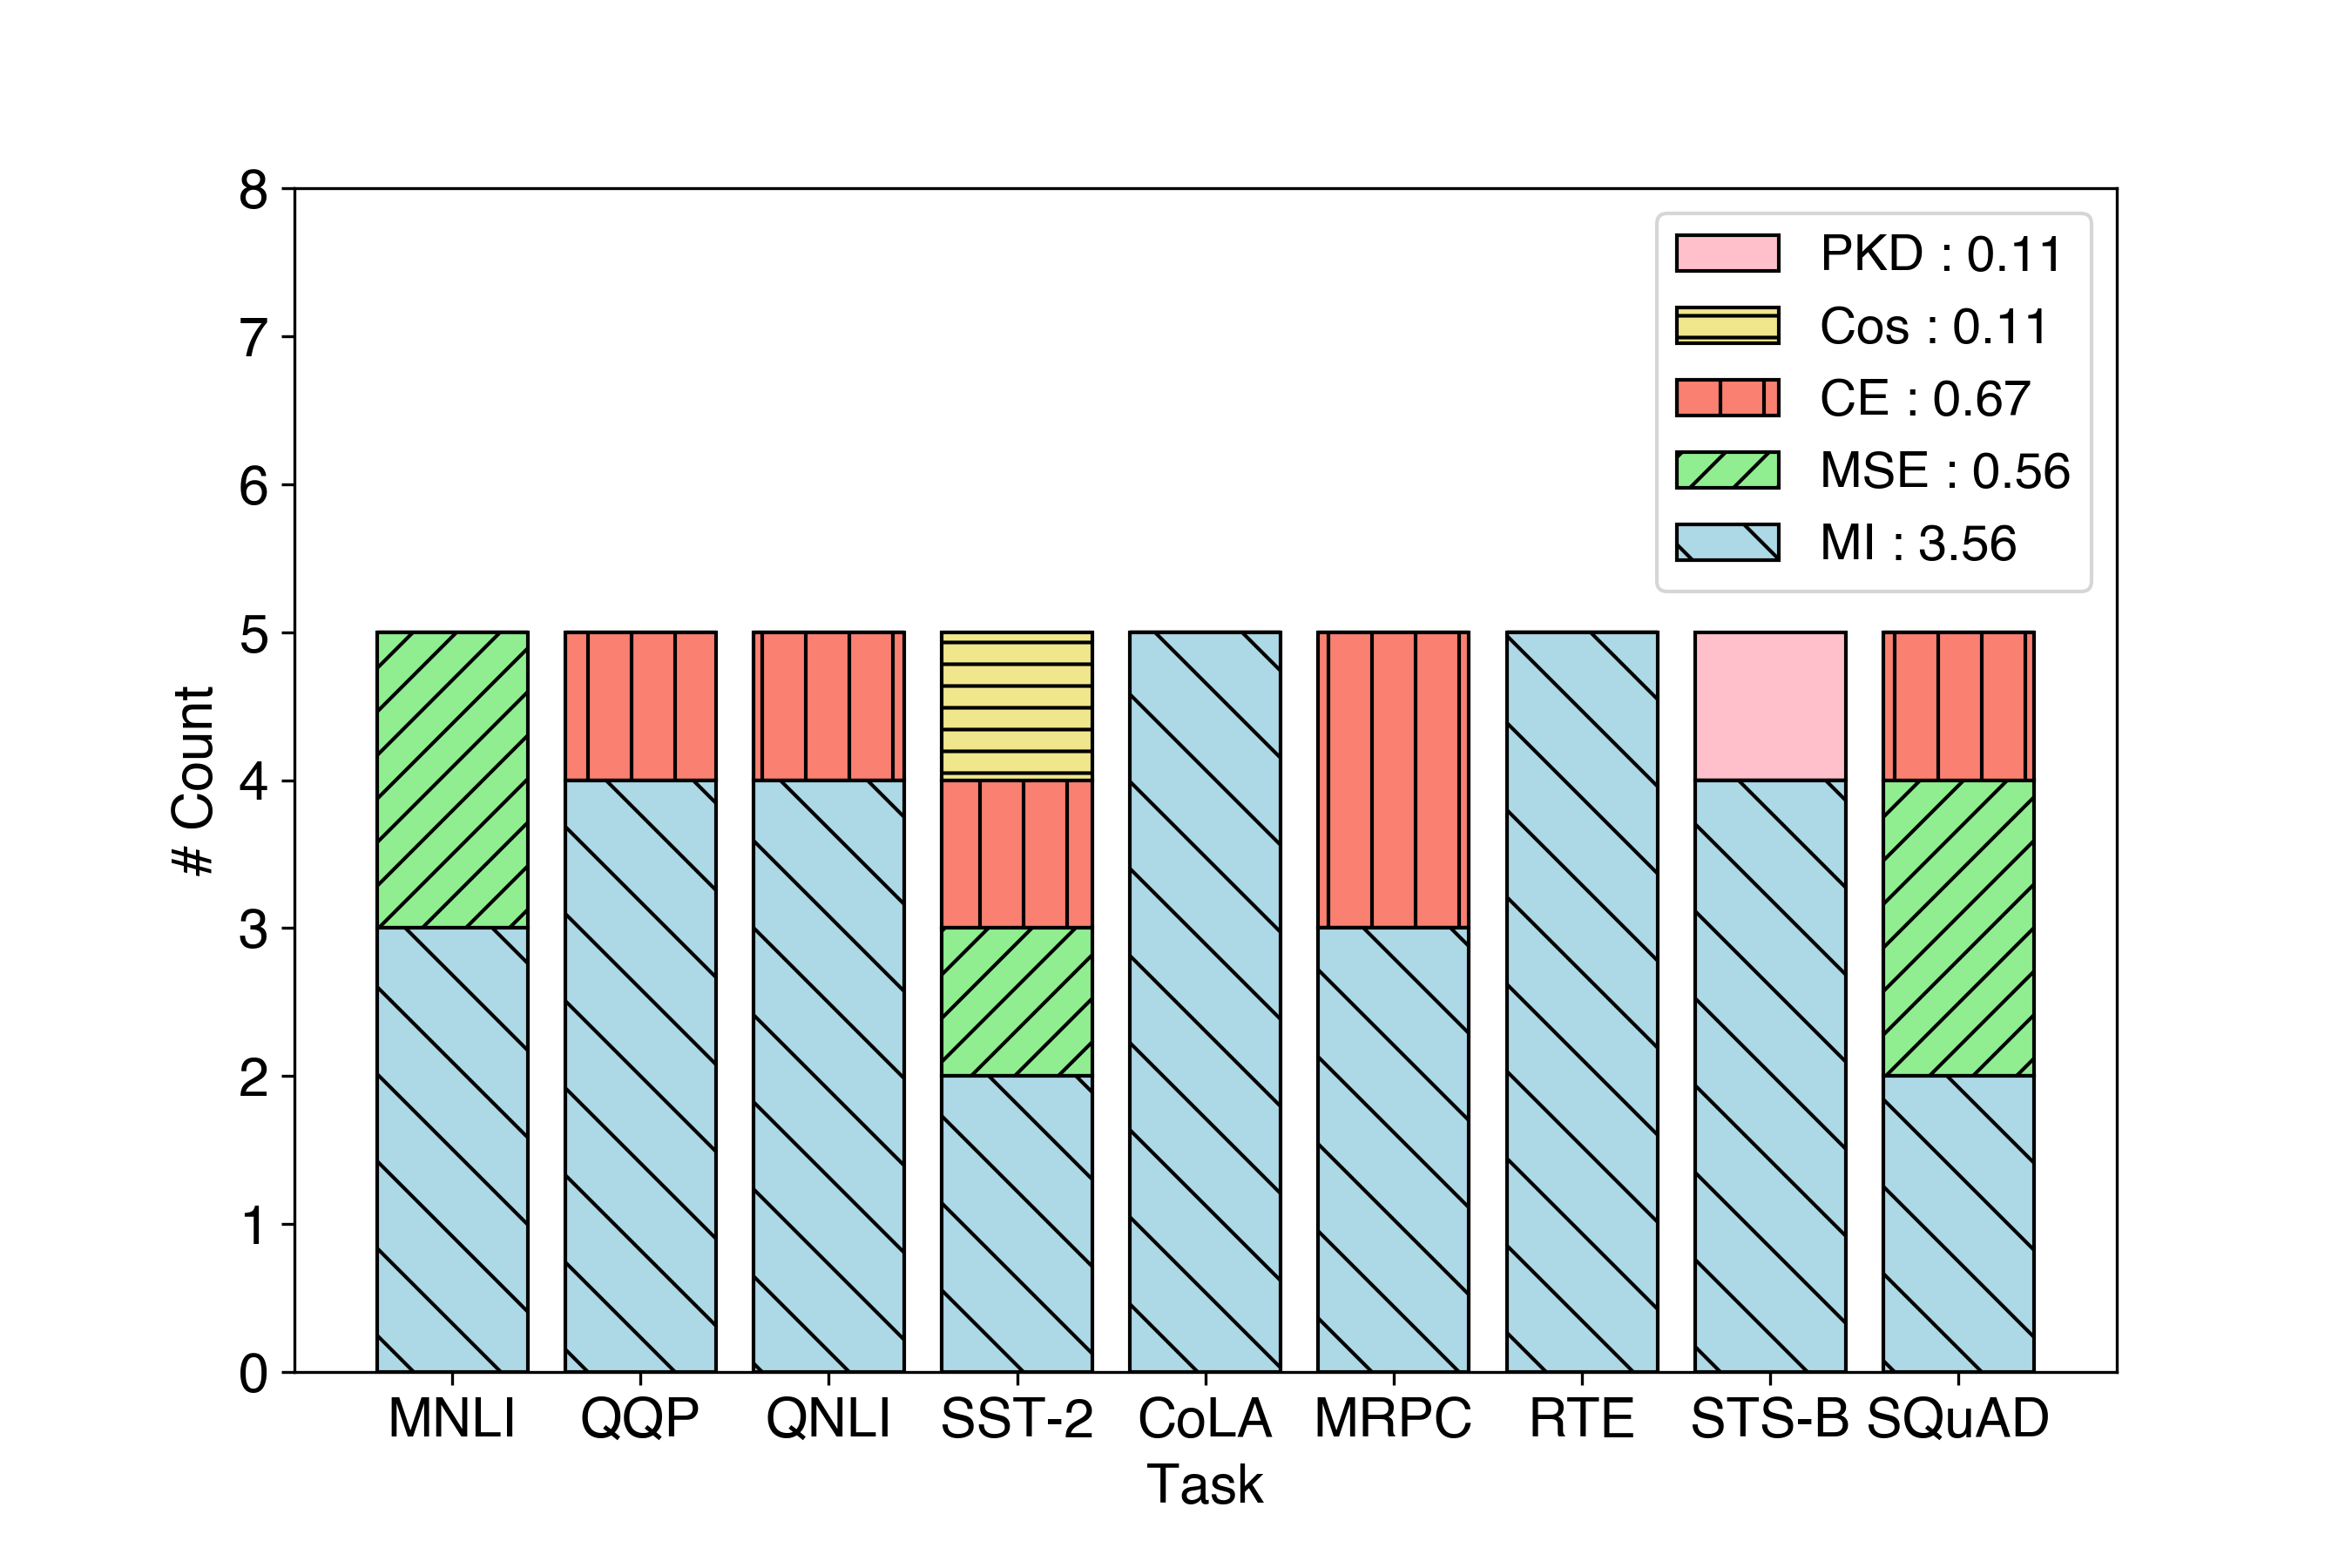
\includegraphics[width=0.8\linewidth]{pics/inter_loss.png}
%   \caption{Intermediate objective functions used in the top-5 performing KD configurations on each dataset. The average count of each objective function is listed in the legend. Configurations are detailed in Appendix.}
%   \label{fig:top5}
% \end{minipage}
% \hfill
% \end{figure*}

\paragraph{More about AutoDistiller} \label{sec:app:task_embedding}
We evaluate the performance of \emph{AutoDistiller} on the 8 GLUE datasets via a leave-one-dataset-out cross-validation protocol. Figure~\ref{fig:leaveoneout} shows that \emph{AutoDistiller} achieves positive Spearman's rank correlation coefficients for most datasets.

\begin{figure}[!tb]
    \centering
  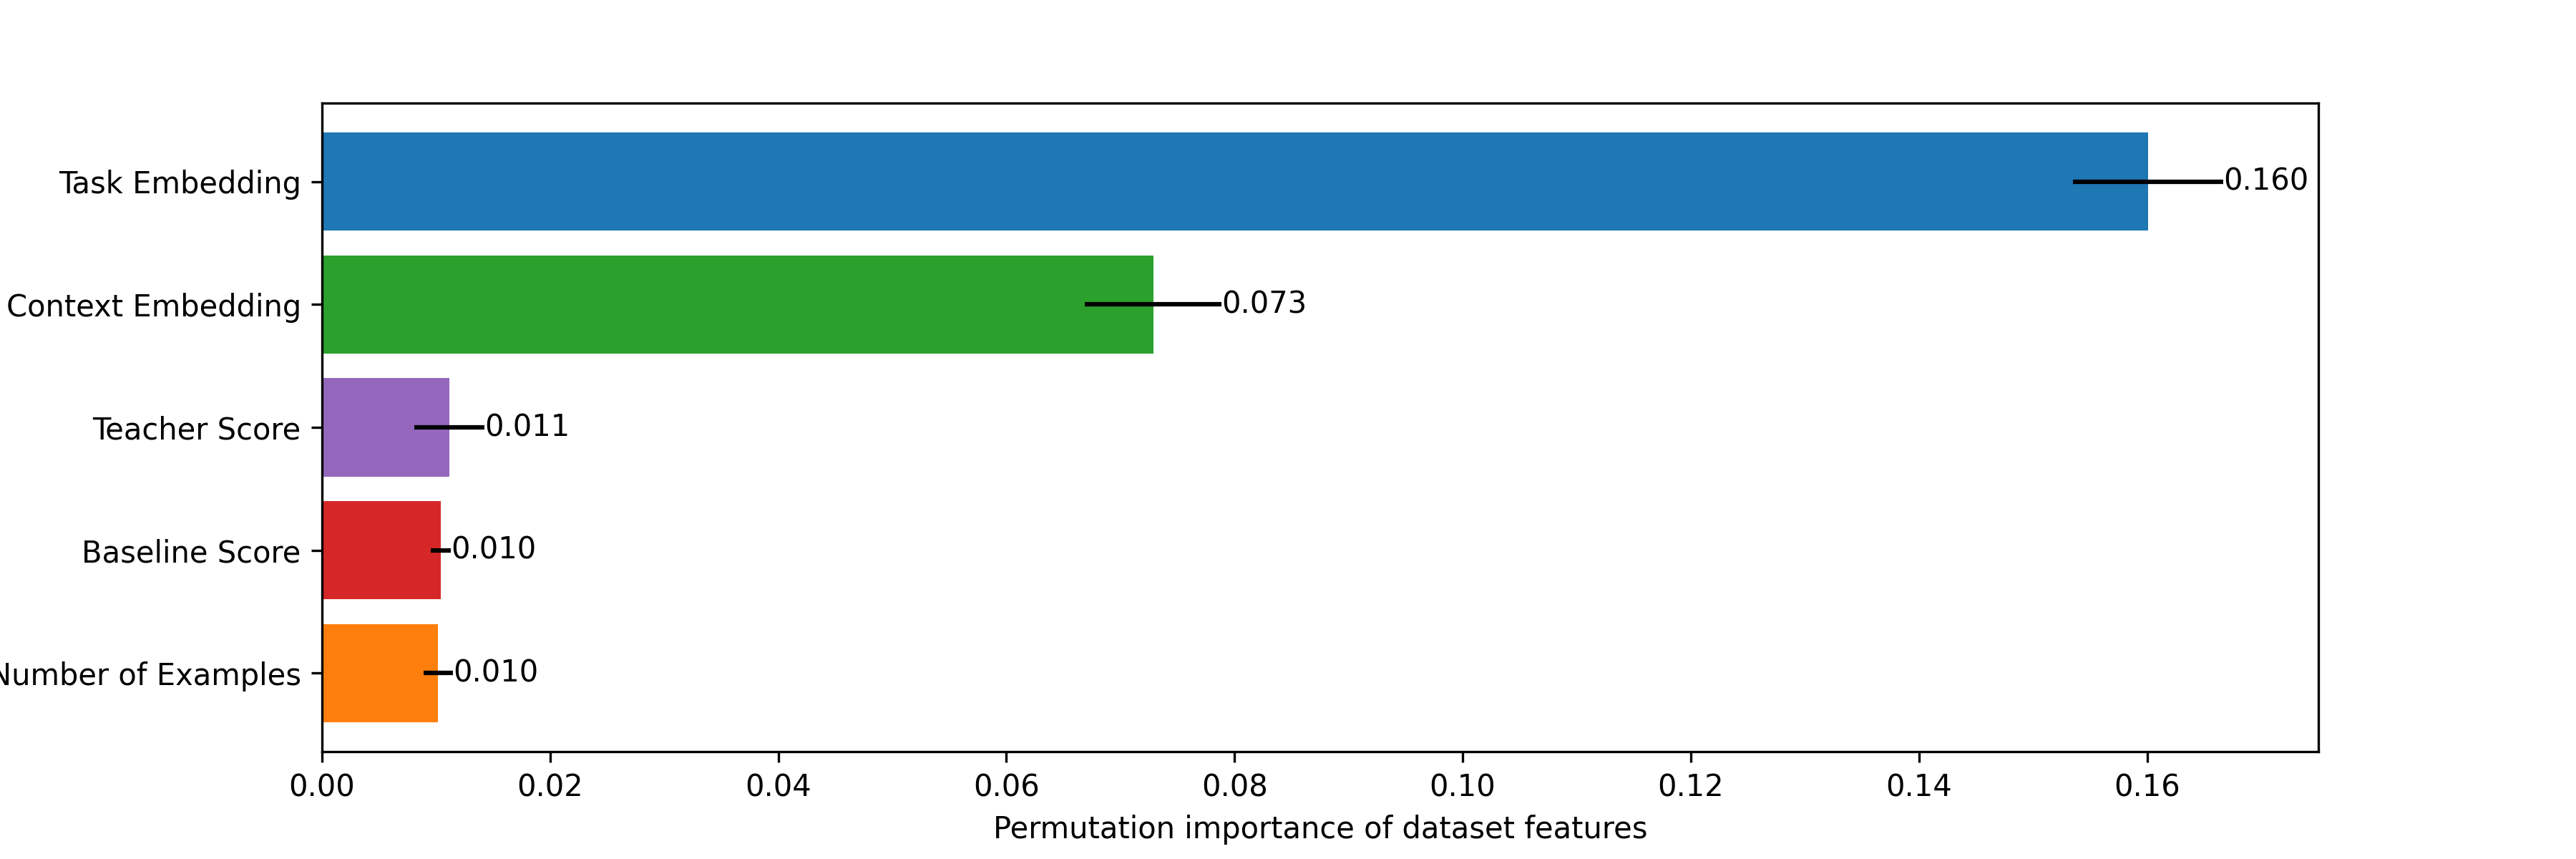
\includegraphics[width=0.6\linewidth]{pics/permutation_importance.png}
  \caption{Permutation importance of the five dataset features.}
  \label{fig:permutation}
\end{figure}
% We extract features of datasets from scratch and represent them as a fixed dimension embedding according to instructions in Table \ref{tab:task_embedding}.  To look into the necessity of these features to \emph{AutoDistiller}, we calculate permutation importance in Figure \ref{fig:permutation}. We observe that all features pertain positive importance, among which the task and context embeddings are the two features with the highest feature importance. Besides, we evaluate the performance of \emph{AutoDistiller} on the 8 GLUE datasets via a leave-one-dataset-out cross-validation protocol. Figure~\ref{fig:leaveoneout} shows that \emph{AutoDistiller} achieves positive Spearman's rank correlation coefficients for most datasets.

% \begin{figure}[!tb]
%     \centering
%     \begin{subfigure}[b]{0.45\textwidth}
%     \centering
%     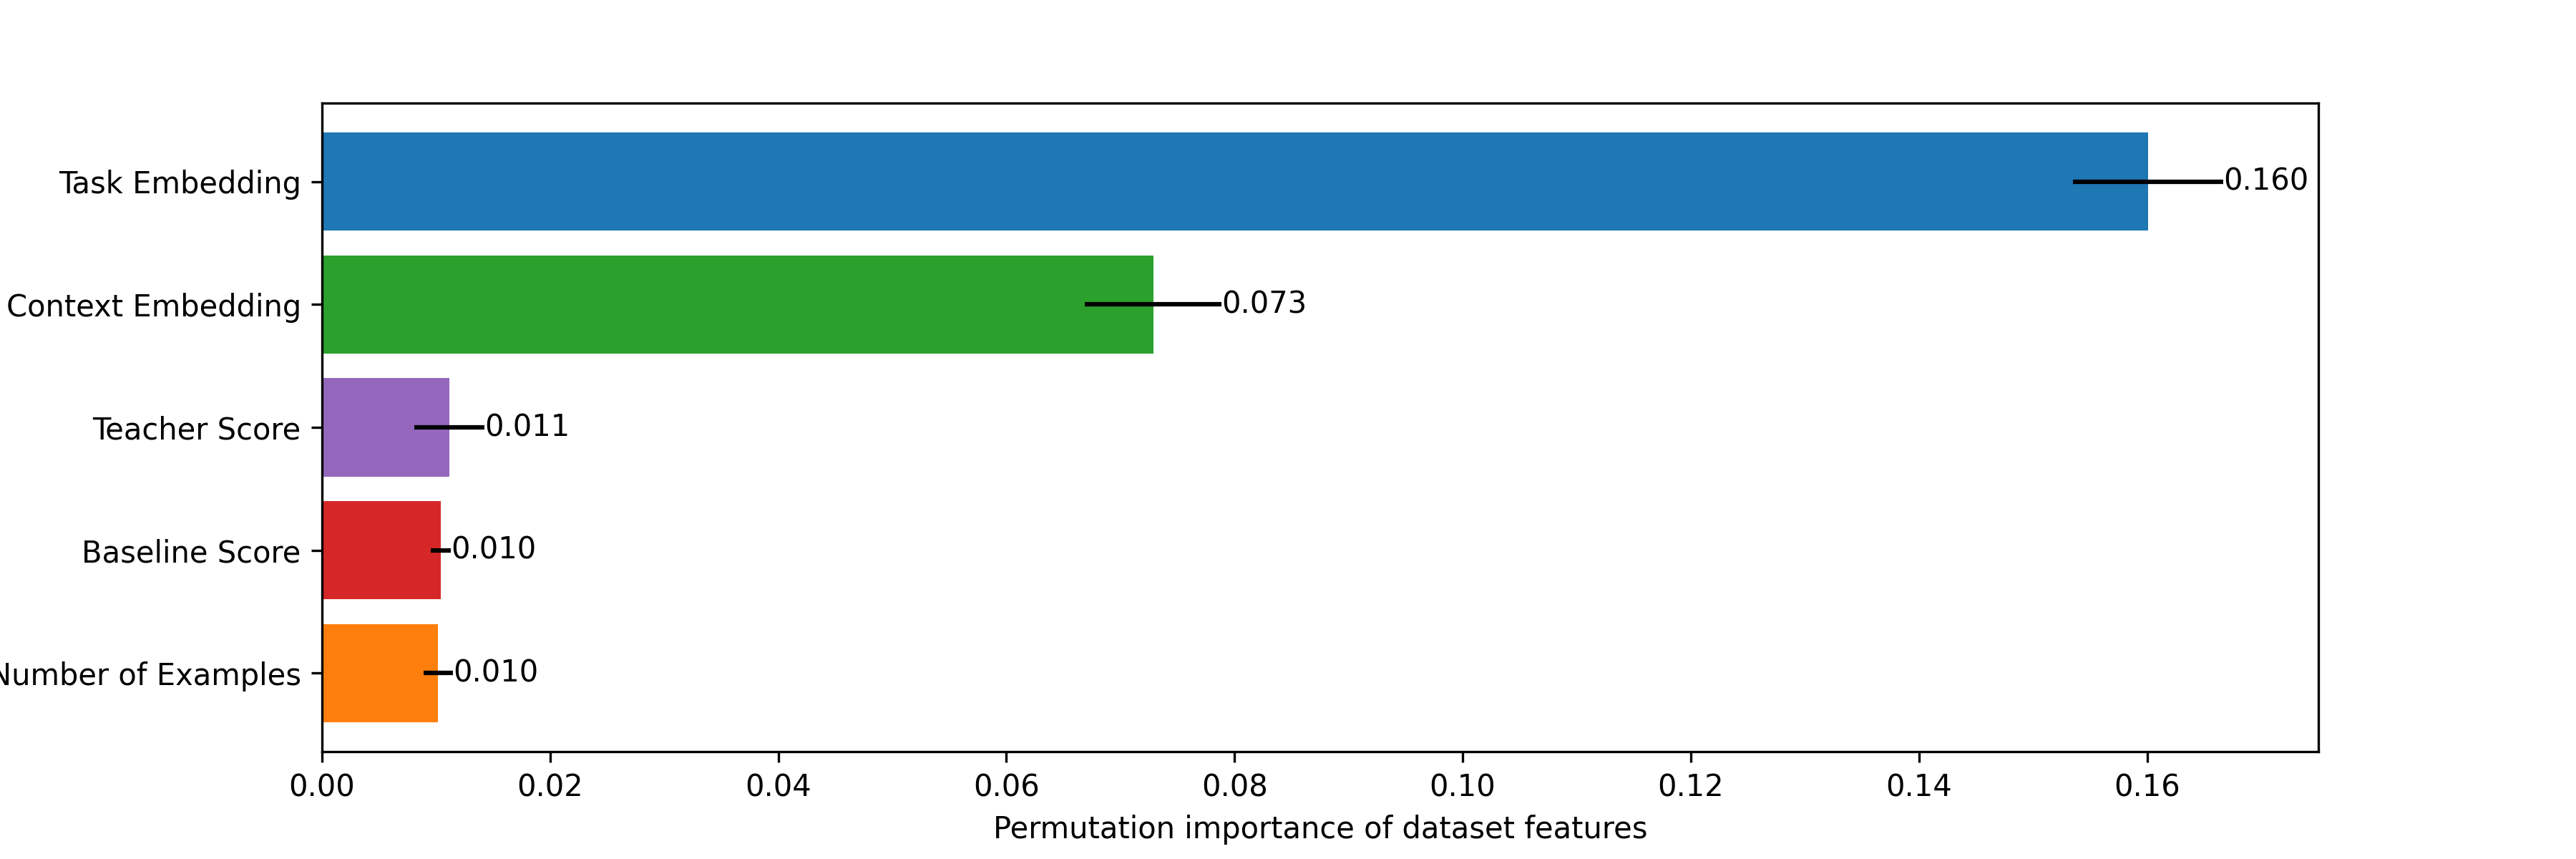
\includegraphics[width=0.8\linewidth]{pics/permutation_importance.png}
%   \caption{}
%   \label{fig:permutation}
%     \end{subfigure}
%     \begin{subfigure}[b]{0.45\textwidth}
% %    \begin{minipage}{6cm}
%     \centering
%     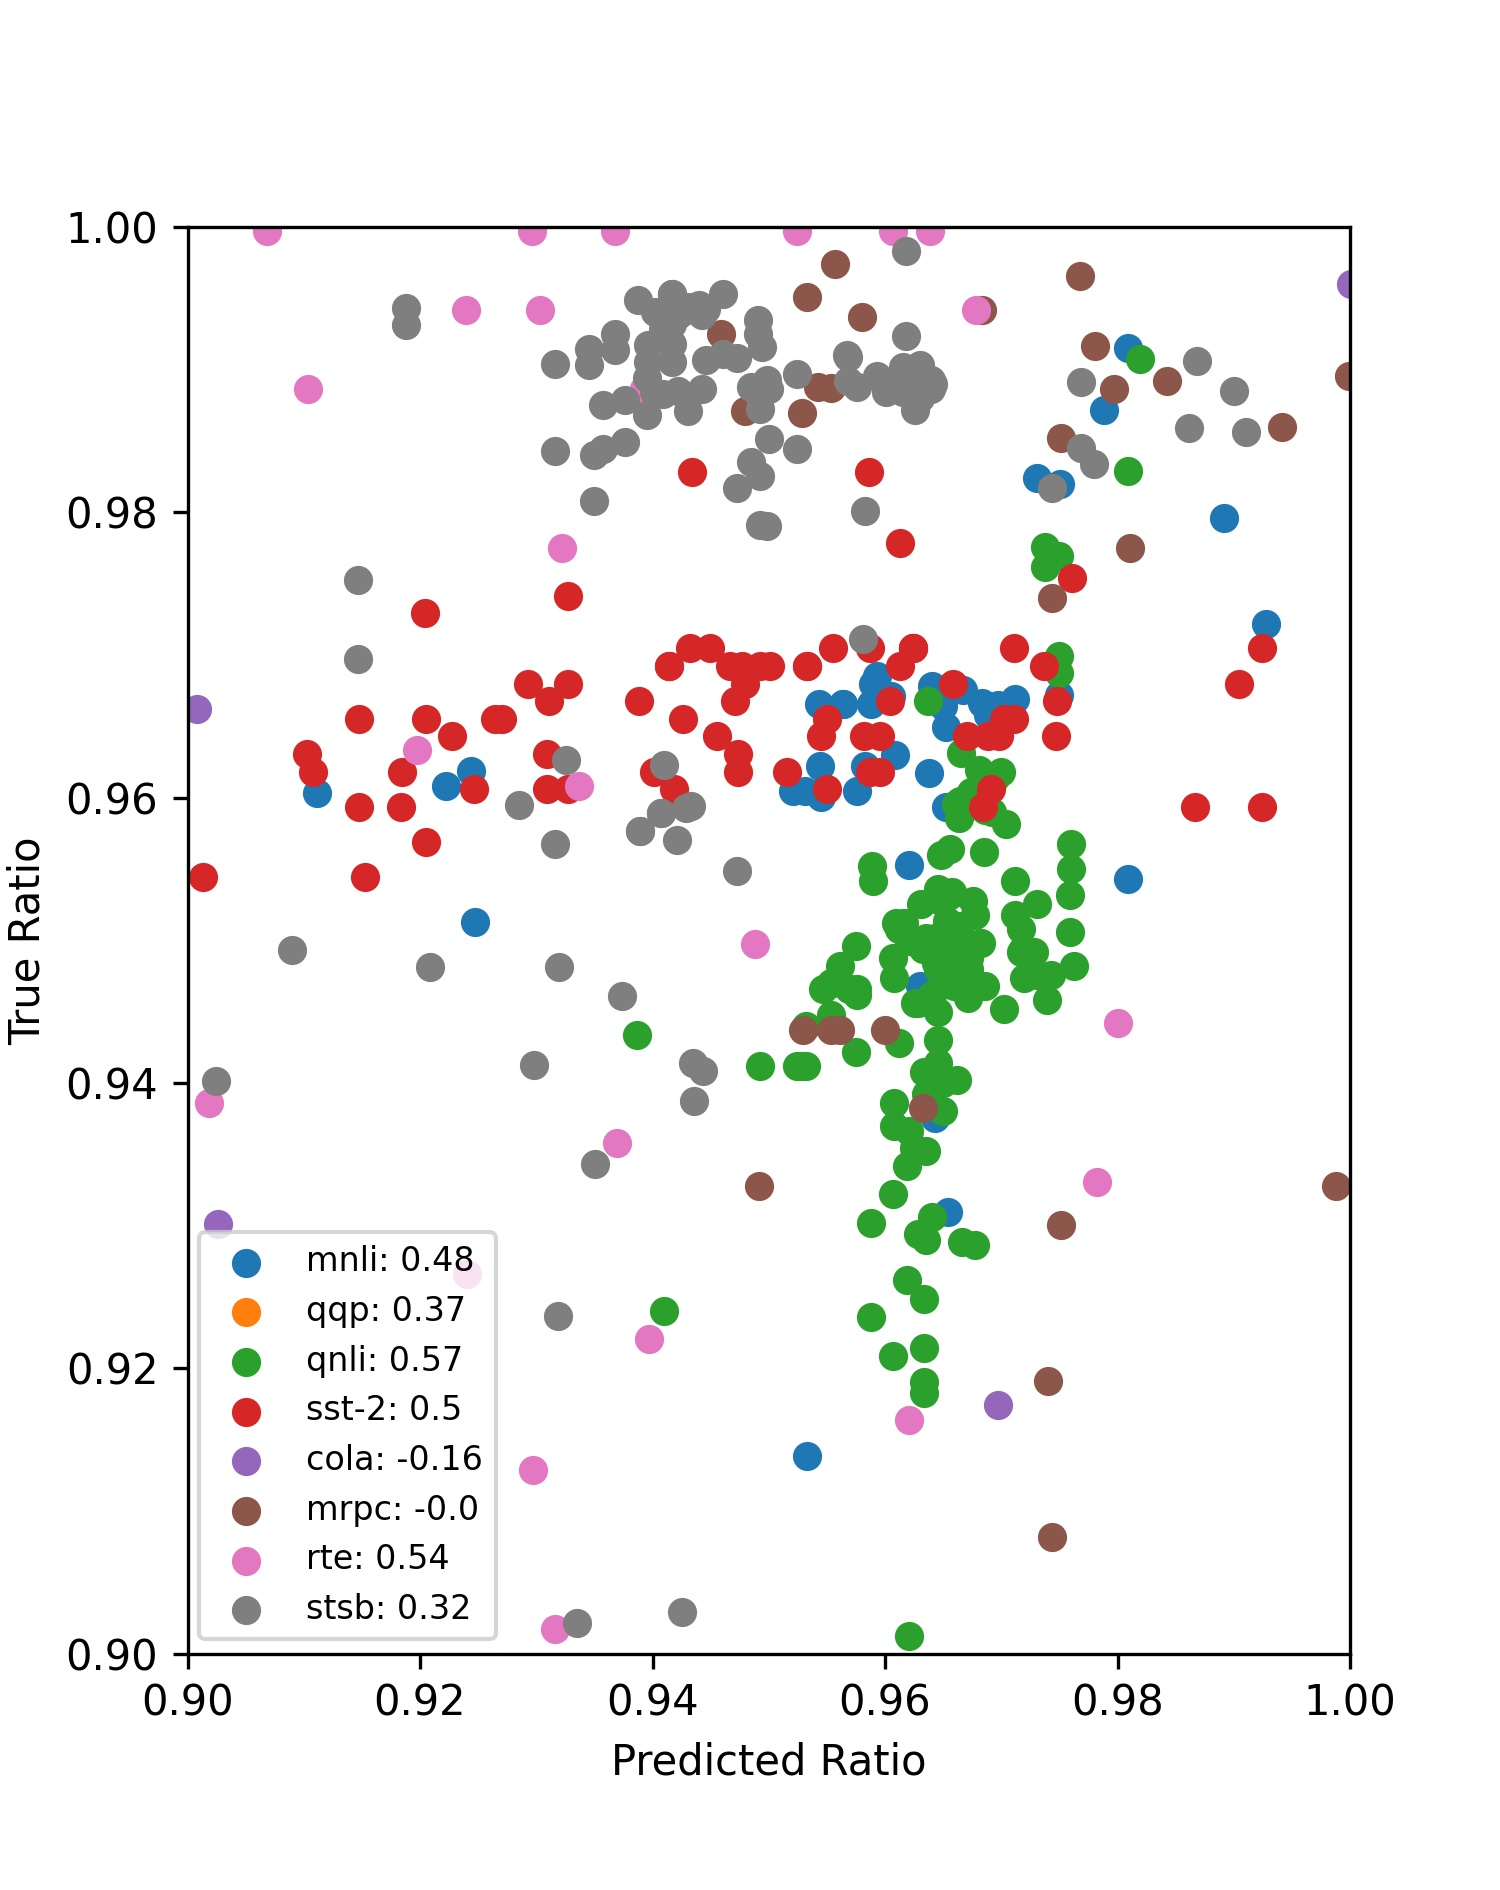
\includegraphics[width=0.6\linewidth]{pics/leave_one_out_predictions_100d.jpg}
%   \caption{
%   }
%   \label{fig:leaveoneout}
%     \end{subfigure}
%     % \caption{Distillation ratio of  \emph{AutoDistiller} (AD) recommended strategies for a fine-tuned $\text{BERT}_\text{BASE}$ teacher and $\text{TinyBERT}_4$ student under two settings. Higher ratio indicates better distillation performance. Mean and standard deviation of the groups of ratios are listed in the legend.}
%     \caption{Figure (a) is the permutation importance of the five dataset features. In Figure (b) we evaluate held-out AutoDistiller predictions on GLUE via leave-one-out estimates. We use dataset-level cross-validation that holds out each GLUE dataset from AutoDistiller training. For each held-out dataset, the legend lists Spearman's rank correlation between the predicted vs.\ actual distillation ratio across different KD pipelines. The average Spearman's rank correlation value across the 8 datasets is 0.33.}
%     \vspace{-1em}
% \end{figure}


\begin{figure}[tb!]
    \centering
    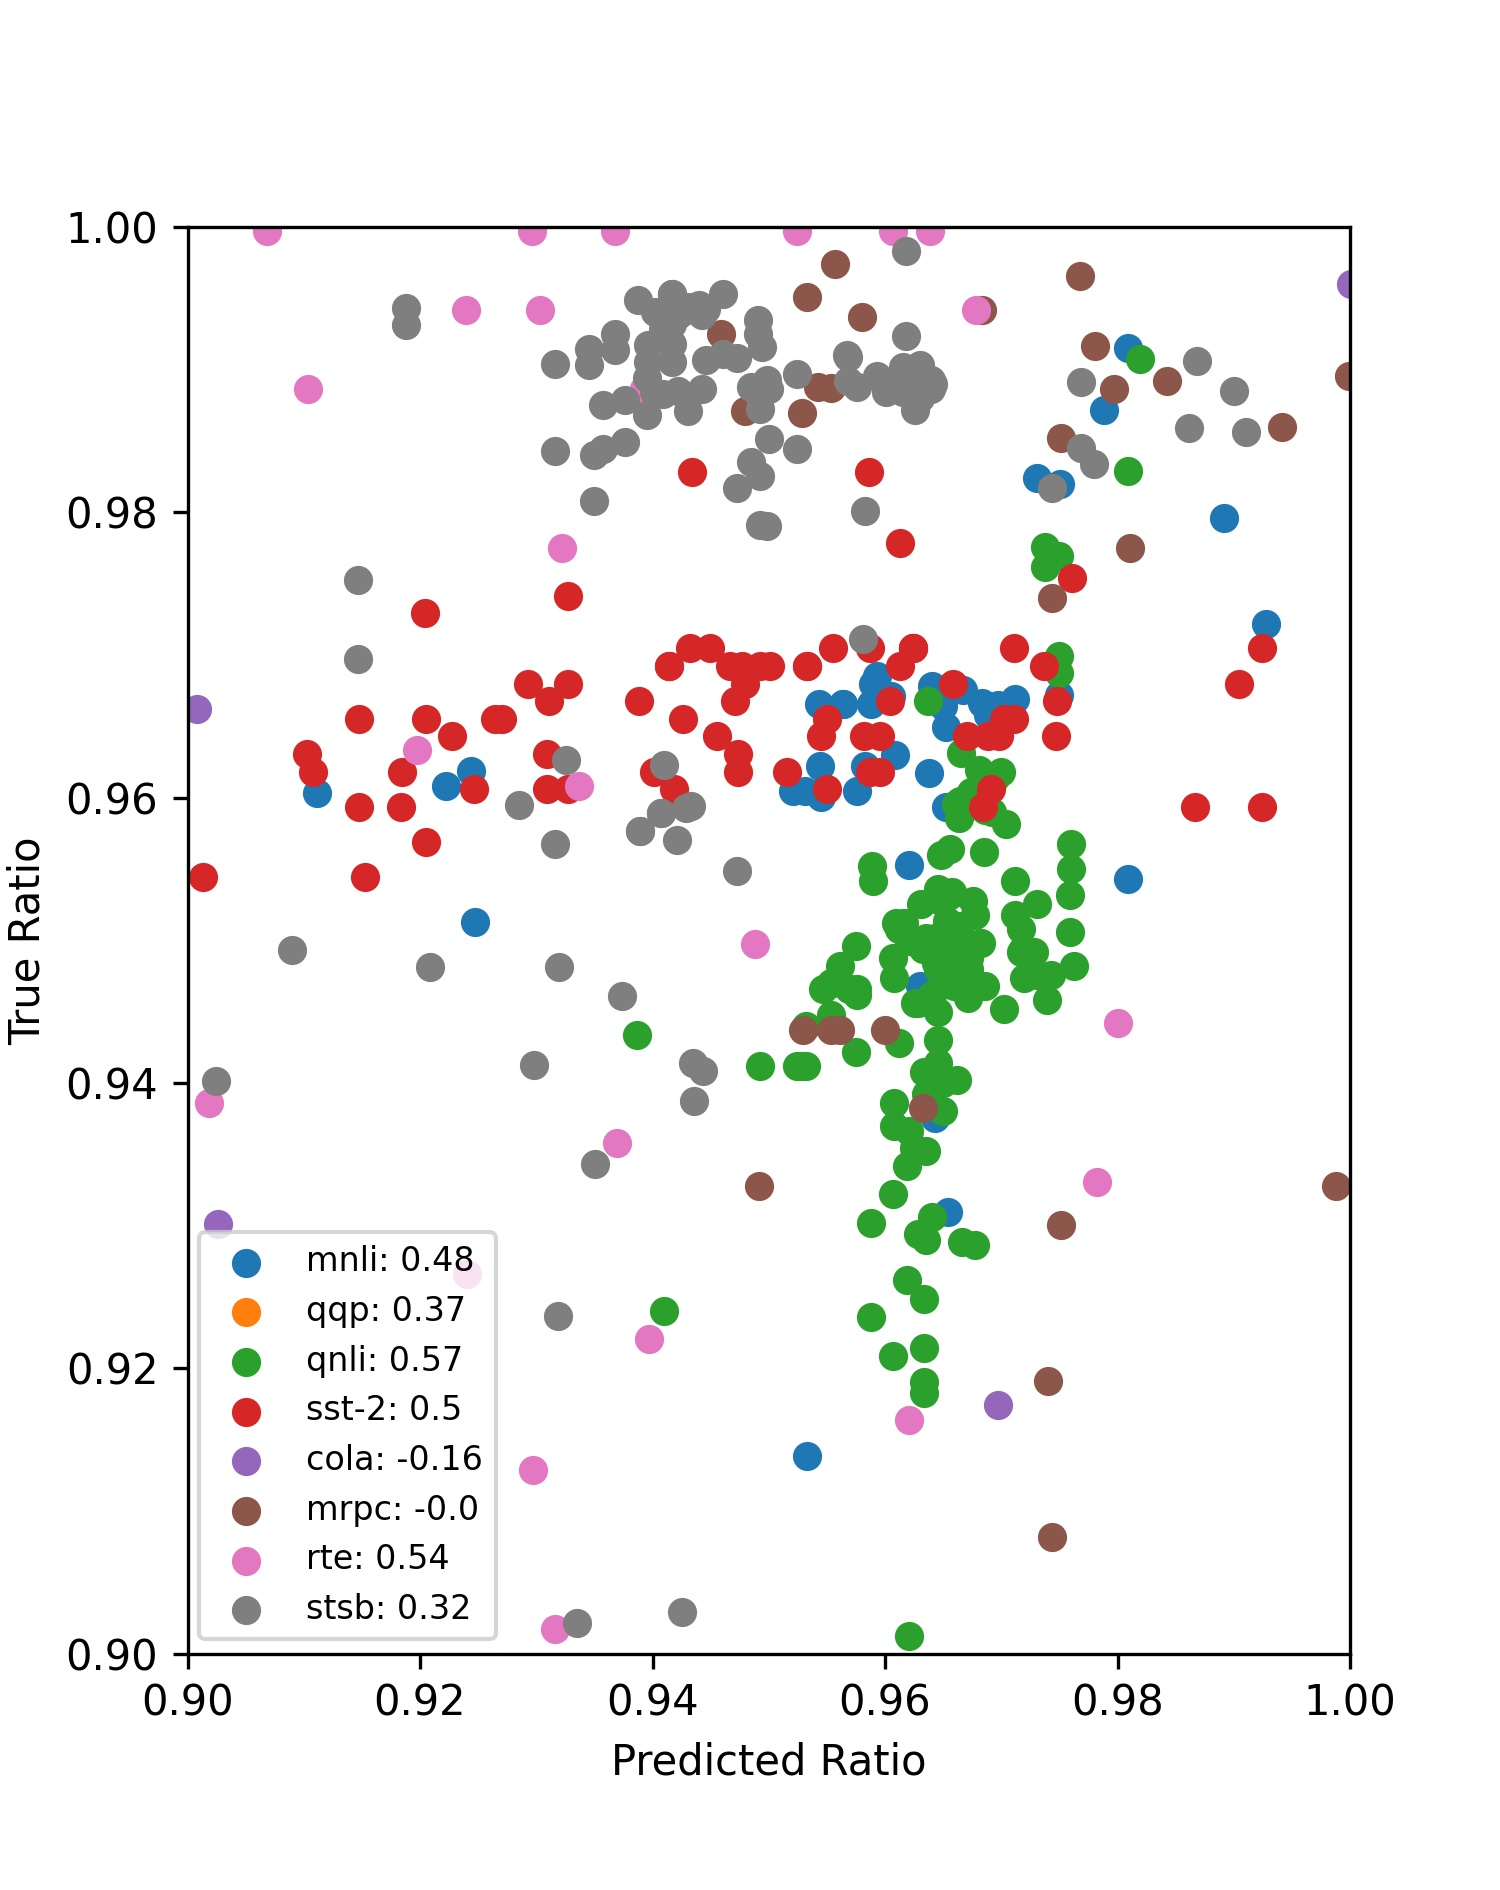
\includegraphics[width=0.5\linewidth]{pics/leave_one_out_predictions_100d.jpg}
  \caption{Evaluating held-out AutoDistiller predictions on GLUE via leave-one-out estimates. We use dataset-level cross-validation that holds out each GLUE dataset from AutoDistiller training. For each held-out dataset, the legend lists Spearman's rank correlation between the predicted vs.\ actual ratio (teacher's performance achieved by student's) across different KD pipelines. The average Spearman's rank correlation value across the 8 datasets is 0.33.
  }
  \label{fig:leaveoneout}
\end{figure}

\clearpage
\section{Top Configurations in Distiller}
\label{sec:app:top-config}
Here we list the top 5 configurations from the Distiller search space that performed best on  each dataset in Table~\ref{tab:top5}.
\begin{table*}[b!]
\centering
\caption{Top 5 configurations to distill a $\text{BERT}_{\text{BASE}}$ teacher to a $\text{TinyBERT}_4$ student on every dataset. To reduce the search space, we only compare configurations that don't use data augmentation. As Hyper-parameter $\alpha$ is only valid for MI-$\alpha$, the value of $\alpha$ is set to N for other intermediate loss in the table.}
\resizebox{0.85\linewidth}{!}{%
\begin{tabular}{lclccll}
\toprule
Task & Intermediate Loss  & $\alpha$ & Layer Mapping Strategy & KD Loss & \#Example & Score \\
\hline \hline
MNLI & MI-$\alpha$ & 0.9 & EMD & MSE & 393000 & 81.7 \\
MNLI & MI-$\alpha$ & 0.1 & EMD & MSE & 393000 & 81.7 \\
MNLI & MI-$\alpha$ & 0.5 & Skip & MSE & 393000 & 81.7 \\
MNLI & MSE & N & EMD & MSE & 393000 & 81.6 \\
MNLI & MSE & N & Skip & MSE & 393000 & 81.6 \\ \hline
QQP & MI-$\alpha$ & 0.9 & EMD & MSE & 364000 & 90.2 \\
QQP & MI-$\alpha$ & 0.1 & EMD & MSE & 364000 & 90.2 \\
QQP & CE & N & Skip & MSE & 364000 & 90.2 \\
QQP & MI-$\alpha$ & 0.1 & EMD & MSE & 364000 & 90.1 \\
QQP & MI-$\alpha$ & 0.1 & Skip & MSE & 364000 & 90.1 \\ \hline
QNLI & CE & N & Last & MSE & 105000 & 87.4 \\
QNLI & MI-$\alpha$ & 0.5 & Skip & MSE & 105000 & 87.4 \\
QNLI & MI-$\alpha$ & 0.5 & Last & CE & 105000 & 87.3 \\
QNLI & MI-$\alpha$ & 0.9 & Skip & CE & 105000 & 87.2 \\
QNLI & MI-$\alpha$ & 0.1 & Skip & CE & 105000 & 87.1 \\
\hline
SST-2 & Cos & N & Last & MSE & 67000 & 90.6 \\
SST-2 & MSE & N & Skip & CE & 67000 & 90.5 \\
SST-2 & MI-$\alpha$ & 0.1 & Last & CE & 67000 & 90.3 \\
SST-2 & CE & N & Skip & MSE & 67000 & 90.3 \\
SST-2 & MI-$\alpha$ & 0.9 & Skip & CE & 67000 & 90.3 \\ \hline
CoLA & MI-$\alpha$ & 0.1 & EMD & MSE & 8500 & 22.3 \\
CoLA & MI-$\alpha$ & 0.5 & EMD & MSE & 8500 & 21.6 \\
CoLA & MI-$\alpha$ & 0.5 & EMD & CE & 8500 & 21.1 \\
CoLA & MI-$\alpha$ & 0.1 & Last & MSE & 8500 & 21.1 \\
CoLA & MI-$\alpha$ & 0.5 & Skip & MSE & 8500 & 21.0 \\ \hline
MRPC & MI-$\alpha$ & 0.1 & EMD & CE & 3700 & 90.3 \\
MRPC & MI-$\alpha$ & 0.5 & EMD & CE & 3700 & 90.2 \\
MRPC & CE & N & Skip & CE & 3700 & 89.9 \\
MRPC & MI-$\alpha$ & 0.9 & EMD & CE & 3700 & 89.9 \\
MRPC & CE & N & Last & MSE & 3700 & 89.7 \\ \hline
RTE & MI-$\alpha$ & 0.1 & Skip & CE & 2500 & 70.8 \\
RTE & MI-$\alpha$ & 0.9 & Skip & CE & 2500 & 70.4 \\
RTE & MI-$\alpha$ & 0.5 & Skip & CE & 2500 & 70.0 \\
RTE & MI-$\alpha$ & 0.1 & Last & CE & 2500 & 70.0 \\
RTE & MI-$\alpha$ & 0.5 & Last & CE & 2500 & 69.3 \\\hline
STS-B & MI-$\alpha$ & 0.9 & Skip & MSE & 7000 & 88.0 \\
STS-B & MI-$\alpha$ & 0.5 & Skip & MSE & 7000 & 88.0 \\
STS-B & MI-$\alpha$ & 0.9 & EMD & MSE & 7000 & 87.9 \\
STS-B & MI-$\alpha$ & 0.1 & Last & MSE & 7000 & 87.9 \\
STS-B & PKD & N & Skip & MSE & 7000 & 87.9 \\
\hline
SQuAD v1.1 & MSE & N & Skip & MSE & 130000 & 72.6 \\
SQuAD v1.1 & CE & N & Skip & MSE & 130000 & 72.4 \\
SQuAD v1.1 & MSE & N & EMD & MSE & 130000 & 72.3 \\
SQuAD v1.1 & MI-$\alpha$ & 0.9 & Skip & CE & 130000 & 71.9 \\
SQuAD v1.1 & MI-$\alpha$ & 0.9 & Skip & CE & 130000 & 71.7 \\
 \bottomrule
\end{tabular}}
\label{tab:top5}
\end{table*} 
\end{document}
